\documentclass[11pt,a4paper]{article}

% ── Packages ──────────────────────────────────────────────
\usepackage[utf8]{inputenc}
\usepackage[T1]{fontenc}
\usepackage[margin=1in]{geometry}
\usepackage{hyperref}
\usepackage{xcolor}
\usepackage{listings}
\usepackage{booktabs}
\usepackage{longtable}
\usepackage{array}
\usepackage{amsmath,amssymb}
\usepackage{enumitem}
\usepackage{fancyhdr}
\usepackage{titlesec}
\usepackage{caption}
\usepackage{subcaption}
\usepackage{mdframed}
\usepackage{natbib}
\usepackage{multirow}
\usepackage{graphicx}

\usepackage{tikz}                                                               
\usetikzlibrary{positioning, arrows.meta, shapes.geometric}                     
             
% ── Colors & Hyperref ─────────────────────────────────────
\definecolor{codebackground}{HTML}{F5F5F5}
\definecolor{codekeyword}{HTML}{0000FF}
\definecolor{codecomment}{HTML}{228B22}
\definecolor{linkcolor}{HTML}{2563EB}

\hypersetup{
    colorlinks=true,
    linkcolor=linkcolor,
    urlcolor=linkcolor,
    citecolor=linkcolor,
    pdftitle={Dynamic Token Merging for Encoder-Only Transformers},
}

% ── Code listing style ────────────────────────────────────
\lstdefinestyle{codestyle}{
    backgroundcolor=\color{codebackground},
    basicstyle=\ttfamily\small,
    keywordstyle=\color{codekeyword}\bfseries,
    commentstyle=\color{codecomment}\itshape,
    breaklines=true,
    keepspaces=true,
    frame=single,
    framerule=0.4pt,
    rulecolor=\color{black!20},
    xleftmargin=1em,
    xrightmargin=0.5em,
    aboveskip=0.8em,
    belowskip=0.6em,
}
\lstset{style=codestyle}

% ── Header/Footer ─────────────────────────────────────────
\pagestyle{fancy}
\fancyhf{}
\fancyhead[L]{\small\leftmark}
\fancyhead[R]{\small CS224N Final Project Report}
\fancyfoot[C]{\thepage}
\renewcommand{\headrulewidth}{0.4pt}

% ── Column types ──────────────────────────────────────────
\newcolumntype{L}[1]{>{\raggedright\arraybackslash}p{#1}}
\newcolumntype{C}[1]{>{\centering\arraybackslash}p{#1}}

% ── Figure paths ──────────────────────────────────────────
\graphicspath{{figures/}{final-project-report/figures/}{deletion_analysis_snli/}}

% ══════════════════════════════════════════════════════════
\begin{document}

% ── Title ─────────────────────────────────────────────────
\begin{center}
    {\LARGE \textbf{Dynamic Token Merging for Encoder-Only\\
    Transformers: Adapting MrT5's Delete Gate to BERT\\
    and XLM-RoBERTa}}\\[1.2em]
    {\large Stanford CS224N Custom Project}\\[1.5em]

    \begin{tabular}{cc}
        \begin{tabular}{c}
            \textbf{Tianhui/Alina Huang}\\
            Department of Computer Science\\
            Stanford University\\
            \texttt{alinah@stanford.edu}
        \end{tabular}
        &
        \begin{tabular}{c}
            \textbf{Hiva Zaad}\\
            Department of Computer Science\\
            Stanford University\\
            \texttt{hiva@stanford.edu}
        \end{tabular}
    \end{tabular}\\[1.2em]

    \begin{tabular}{c}
        \textbf{Aronima Dass}\\
        Department of Computer Science\\
        Stanford University\\
        \texttt{adass@stanford.edu}
    \end{tabular}\\[0.8em]

    \small \textbf{Mentor: Julie Kallini} \quad \emph{kallini@stanford.edu}\\[0.2em]
    \small \textbf{Sharing:} This report may be posted on the CS224N website.\\[0.2em]
    \small \textbf{Code:} \url{https://github.com/HivaMohammadzadeh1/CS224N-project/tree/main}
\end{center}

\bigskip

% ══════════════════════════════════════════════════════════
\begin{abstract}
Transformer-based language models apply uniform computation to every input token, regardless of token informativeness.
The MrT5 paper \citep{kallini2024mrt5} introduced a \emph{Dynamic Token Merging} (DTM) delete gate for byte-level encoder-decoder models, achieving up to 60\% sequence length reduction with minimal perplexity degradation.
We ask: does this mechanism generalise to subword-based encoder-only architectures used for discriminative NLU?
We implement \textbf{MrBERT} and \textbf{MrXLMR}, adapting the MrT5 delete gate to BERT-base and XLM-RoBERTa-base respectively.
Our gate fires after encoder layer~3 (out of~12), uses a PI controller to hit a target deletion rate~$\delta$, and introduces a novel \emph{pre-deletion blending} mechanism that makes extractive QA viable under token deletion.
Evaluated across six tasks --- SNLI, SQuAD, SST-2, MRPC, IMDB, and TyDi~QA --- our results show:
MrBERT at 30\% deletion achieves \textbf{90.21\%} SNLI accuracy (only 0.27pp below baseline) at \textbf{1.89$\times$} A100 inference speedup;
SST-2 drops by only 0.62pp (97.29\%$\to$96.67\%), while MRPC shows a larger 17.32pp drop, revealing dataset-specific sensitivity;
TyDi~QA span EM recovers from 0.10 (no blending) to 0.35 (layer~9 + blending), matching BERT end accuracy.
A random-deletion baseline scores 2.95pp below MrBERT-30\% on SNLI, confirming learned token selection.
Beyond efficiency, the gate acts as an \emph{attention-sparsifying regulariser}, preferentially pruning function words while preserving content-bearing tokens.
MrXLMR achieves 82.27\% on SNLI at 30\% deletion (baseline 89.85\%), suggesting XLM-R's higher per-token information density requires more conservative deletion strategies.
\end{abstract}


% ══════════════════════════════════════════════════════════
\section{Introduction}
\label{sec:introduction}

Large pretrained transformers such as BERT \citep{devlin2019bert} and XLM-RoBERTa \citep{conneau2020xlmr} achieve state-of-the-art performance across a wide range of NLU tasks. However, their computational cost scales quadratically with sequence length due to self-attention, making inference expensive. A natural question is whether all tokens are equally important for a given task: for a sentiment classification example, function words like ``the'' and ``of'' carry little discriminative content, while content words like ``terrible'' or ``outstanding'' are crucial.

The MrT5 paper \citep{kallini2024mrt5} proposes \emph{Dynamic Token Merging} (DTM): a learned scalar gate inserted after an early encoder layer that assigns each token a deletion score. Low-scoring tokens are masked out of subsequent attention computations (soft deletion) or physically removed (hard deletion). MrT5 demonstrates this on a byte-level T5 model, showing up to 60\% sequence reduction at minimal perplexity cost.

We address the open question: \textbf{does this mechanism transfer to subword-based encoder-only models trained on discriminative NLU tasks?} The transfer is non-trivial because:

\begin{enumerate}[nosep]
    \item BERT and XLM-R use subword tokenisation, not byte-level tokens, so token granularity and importance distributions differ.
    \item Encoder-only models pool to a single \texttt{[CLS]} vector for classification, creating a different information-flow bottleneck than encoder-decoder models.
    \item Extractive QA requires localising answer spans: answer tokens must survive deletion --- a hard constraint absent in language modelling.
    \item XLM-R spans 100 languages with a shared 250K SentencePiece vocabulary; importance patterns must generalise across scripts.
\end{enumerate}


\noindent Our contributions are:
\begin{itemize}[nosep]
    \item \textbf{MrBERT}: BERT-base with a MrT5-style delete gate, evaluated on SNLI, SST-2, MRPC, IMDB, SQuAD, and TyDi~QA.
    \item \textbf{MrXLMR}: XLM-RoBERTa-base with the same mechanism, evaluated on SNLI.
    \item \textbf{Pre-deletion blending}: a novel mechanism enabling extractive QA under deletion; span EM improves 3.5$\times$.
    \item \textbf{Comprehensive ablations}: PI controller necessity, gate layer placement (layers 1/3/6/9), soft vs.\ hard deletion gap, and deletion pattern analysis.
\end{itemize}


% ══════════════════════════════════════════════════════════
\section{Background and Related Work}
\label{sec:related-work}

\textbf{MrT5} \citep{kallini2024mrt5}. The direct antecedent of this work. MrT5 attaches a scalar delete gate after a selected encoder layer of a T5-based byte-level model. A PI controller adjusts the deletion loss coefficient~$\alpha$ to track a target deletion rate. The gate adds fewer than 3K parameters to a 250M parameter model, achieving 50--60\% sequence reduction on language modelling tasks with minimal degradation.

\textbf{Efficient transformers.} Sparse attention methods (Longformer, BigBird) reduce attention from $O(n^2)$ to $O(n)$. Low-rank approaches (Linformer) and kernel methods (Performer) approximate the full attention matrix. Early-exit approaches (DeeBERT, PABEE) skip later layers for easy examples. Token pruning methods (TR-BERT, SpAtten, LTP) learn to drop tokens, often requiring reinforcement learning. Unlike these, our method keeps the network depth fixed but reduces the number of tokens processed in later layers, trained end-to-end with differentiable soft deletion and requiring no architectural changes beyond the gate module.

\textbf{Token importance and robustness.} \citet{michel2019heads} and \citet{voita2019heads} showed many BERT attention heads are redundant. \citet{clark2019attention} found BERT attention aligns with syntactic structure; function words receive less attention in higher layers, consistent with our gate's deletion patterns (Section~\ref{sec:deletion-patterns}). Our delete gate can also be viewed as a form of structured, learned subword regularisation, analogous to BPE-dropout: by stochastically removing low-value tokens during training, it may improve classification robustness on redundant tasks (Section~\ref{sec:task-sensitivity}).

\textbf{Summary of differences.} Our work differs from prior token pruning by: (1)~applying dynamic merging to encoder-only architectures; (2)~using a PI controller to stabilise deletion in a discriminative setting; (3)~introducing pre-deletion blending for extractive QA; and (4)~providing multi-task analysis (including cross-lingual QA) to identify where merging helps or hurts.



% ══════════════════════════════════════════════════════════
\section{Approach}
\label{sec:approach}

\subsection{Architecture Overview}

MrBERT is a pretrained BERT-base encoder with a lightweight delete gate inserted after a selected layer. The gate uses hidden states from that layer to compute a scalar score per token; the score is then used to mask tokens in all subsequent layers.


\begin{figure}[t]                                                 
  \centering                                                        
  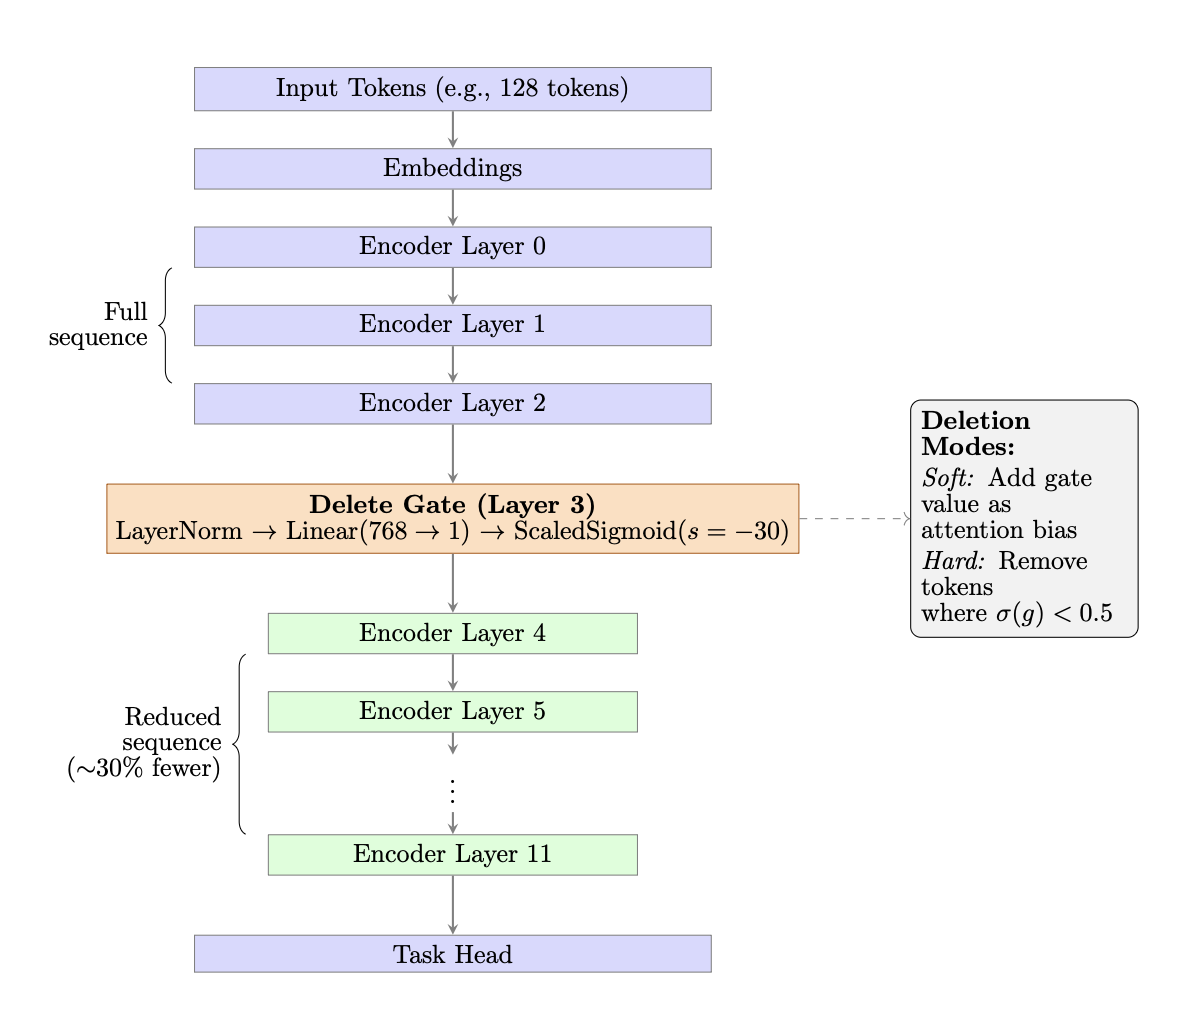
\includegraphics[width=0.7\linewidth]{figures/architecture.png}                           
  \caption{MrBERT architecture overview. The delete gate at layer 3 
  reduces the sequence length for subsequent layers.}               
  \label{fig:mrbert-arch}                                           
  \end{figure}

\textbf{BERT-base} \citep{devlin2019bert}: 12 layers, $d_{\text{model}}=768$, 12 heads, 110M parameters, WordPiece 30K vocabulary. \textbf{XLM-RoBERTa-base} \citep{conneau2020xlmr}: same dimensions, 277M parameters, SentencePiece 250K vocabulary.


\subsection{Delete Gate}
\label{sec:delete-gate}

The gate module (\texttt{SigmoidDeleteGate}) has three components:

\textbf{(1) LayerNorm.} The hidden state $\mathbf{h}_i$ from layer \texttt{delete\_gate\_layer} is normalised before projection, stabilising training.

\textbf{(2) Linear projection.} $z_i = \mathbf{W}\mathbf{h}_i + b$, with $\mathbf{W}\sim\mathcal{N}(0,0.02)$ and $b=10.0$. The large positive bias initialises the gate near zero deletion ($g\approx-0.001$), so the model starts from the pretrained baseline.

\textbf{(3) Scaled sigmoid.}
\begin{equation}
    g_i = s \cdot \sigma(-z_i), \qquad s = -30
    \label{eq:scaled-sigmoid}
\end{equation}
Gate values lie in $(-30,0)$: near~$0$ means keep, near~$-30$ means delete. Deletion threshold $\tau = s/2 = -15$. The gate adds only 2,305 parameters ($768+1$ weights $+$ $2{\times}768$ LayerNorm). \texttt{[CLS]}/\texttt{[SEP]} are always kept; \texttt{[PAD]} is always deleted.

\begin{figure}[t]
  \centering
  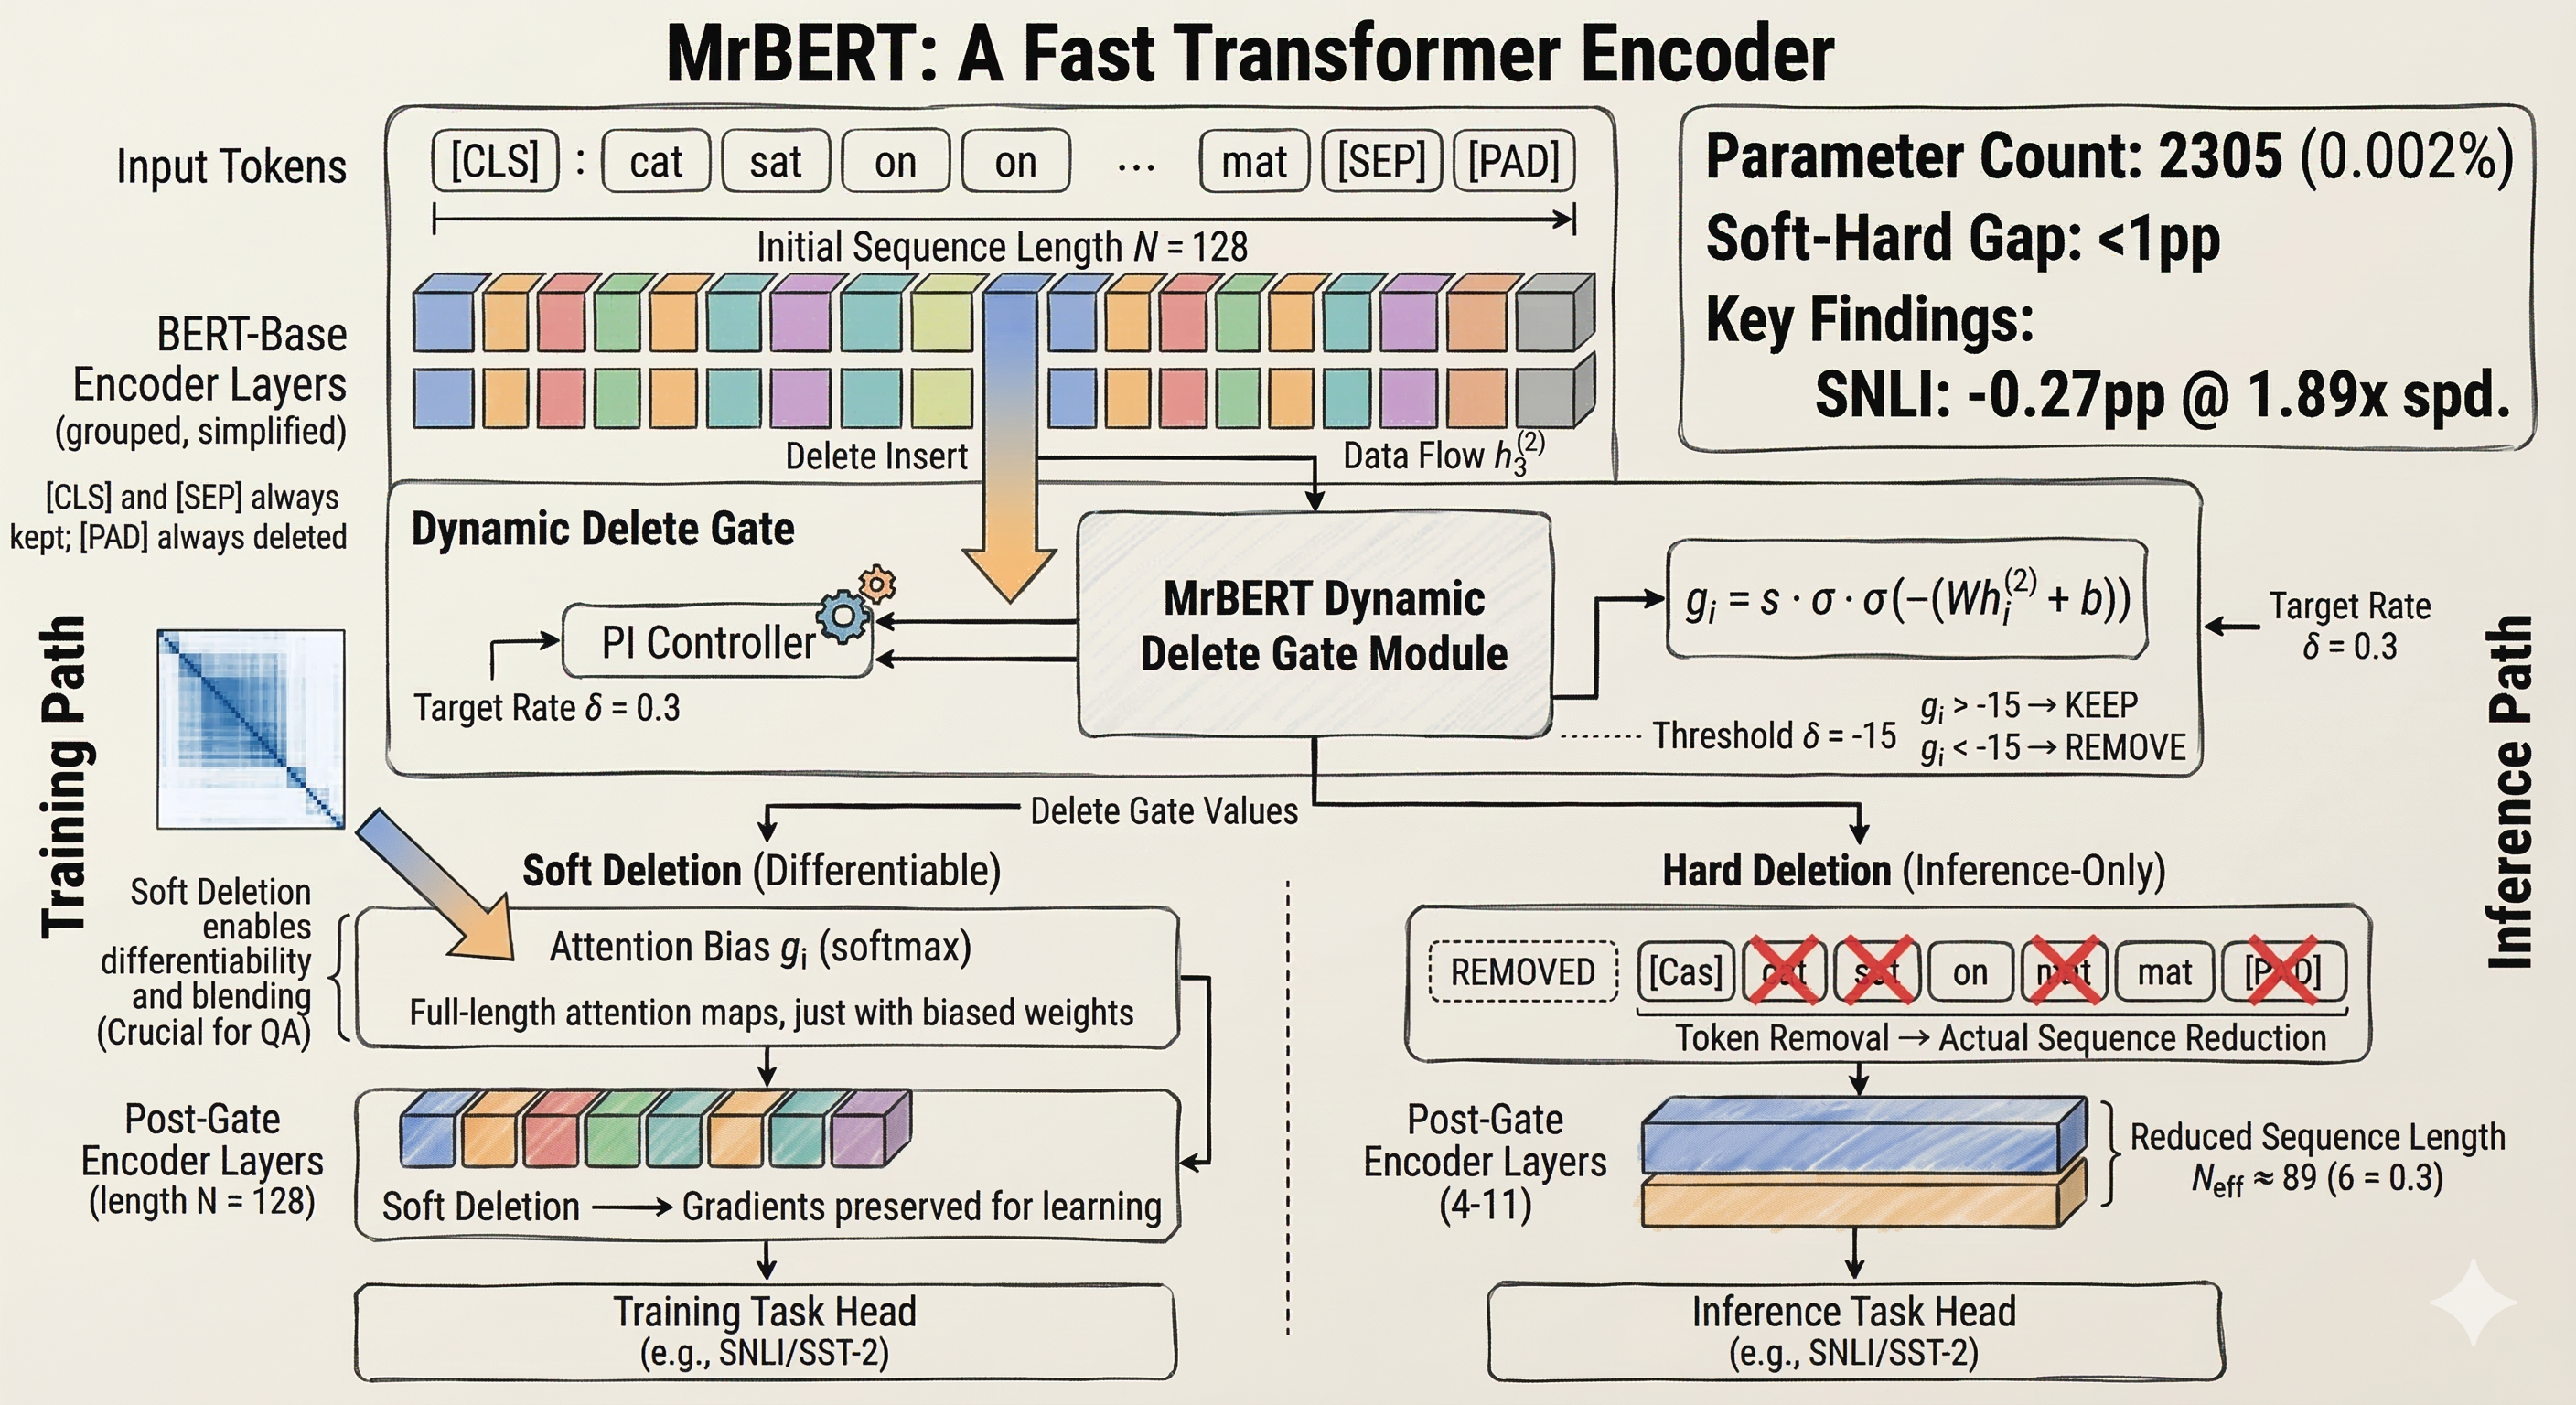
\includegraphics[width=0.7\linewidth]{figures/architecture2.png}
  \caption{Layer-level view of MrBERT. Encoder layers 0--2 (blue) process the full sequence; the delete gate fires after layer~3 (orange), and layers 4--11 (green) operate on the reduced sequence ($\sim$30\% fewer tokens at $\delta{=}0.3$). Soft deletion adds gate values as attention biases; hard deletion physically removes tokens where $g < \tau$.}
  \label{fig:mrbert-layers}
\end{figure}


\subsection{Soft and Hard Deletion}

During training, \textbf{soft deletion} adds $g_i$ as an attention bias:
\begin{equation}
    \tilde{a}(q, k_i) = a(q, k_i) + g_i
\end{equation}
Deleted tokens ($g_i\approx-30$) contribute negligible attention weight, while remaining differentiable for end-to-end training. We additionally apply softmax1 \citep{kallini2024mrt5}:
\begin{equation}
    \text{softmax1}(\mathbf{x})_i = \frac{\exp(x_i)}{1 + \sum_j \exp(x_j)}
    \label{eq:softmax1}
\end{equation}
The extra~$1$ in the denominator allows attention weights to sum to less than~1 when all keys carry large negative gate biases, preventing the model from being forced to attend to deleted tokens.


At inference, \textbf{hard deletion} physically removes positions where $g_i<\tau$, achieving real memory and compute savings.


\subsection{Pre-Deletion Blending}
\label{sec:pre-deletion-blending}

For extractive QA, deleted answer tokens produce corrupted representations at the task head. We introduce \textbf{pre-deletion blending}: for each token~$i$, blend weight $w_i = \text{clamp}(-g_i/30,0,1)$, and:
\begin{equation}
    \tilde{\mathbf{h}}_i = (1-w_i)\cdot\mathbf{h}_i^{(L)} + w_i\cdot\mathbf{h}_i^{(\text{gate})}
    \label{eq:blending}
\end{equation}
where $\mathbf{h}_i^{(L)}$ is the layer-11 output and $\mathbf{h}_i^{(\text{gate})}$ is the pre-gate hidden state. For kept tokens ($w_i\approx0$), the representation is unchanged. For deleted tokens ($w_i\approx1$), it falls back to the richer pre-gate representation. This also provides a gradient signal through deleted positions, preventing gate collapse during QA training (Section~\ref{sec:results-tydiqa}).

\subsection{QA Span Remapping under Hard Deletion}
\label{sec:span-remapping}

Under hard deletion, the span head operates on a shortened sequence. Predicted start and end indices must be remapped to the original tokenisation for correct evaluation. We maintain a per-example mapping $\texttt{keep\_indices}[b,j]$, recording the original position of the $j$-th kept token in example~$b$, along with $\texttt{kept\_lengths}[b]$. After the span head predicts $(\hat{s},\hat{e})$ in the shortened sequence, we recover original-space positions:
\begin{equation}
    s = \texttt{keep\_indices}[b,\hat{s}], \quad e = \texttt{keep\_indices}[b,\hat{e}]
    \label{eq:span-remap}
\end{equation}
Exact Match is then computed in the original token space. Variable-length sequences within a batch are handled via \texttt{torch.gather} with length masks, producing fixed-shape tensors compatible with standard batched inference.


\subsection{PI Controller}
\label{sec:pi-controller}

A PI controller dynamically adjusts the deletion loss coefficient $\alpha$ to track target deletion rate $\delta$:
\begin{align}
    e_t &= \delta - r_t, \quad
    p_t = \gamma p_{t-1} + (1-\gamma)k_p e_t, \quad
    i_t = i_{t-1} + k_i e_t, \quad
    \alpha_t = \max(0, p_t+i_t)
\end{align}
Total loss: $\mathcal{L} = \mathcal{L}_{\text{task}} + \alpha_t\cdot\mathcal{L}_{\text{deletion}}$, where $\mathcal{L}_{\text{deletion}} = \text{mean}(g_i)$ over non-padding tokens. Parameters: $k_p=0.01$, $k_i=10^{-5}$, $\gamma=0.9$.


\subsection{Key Differences from MrT5}

\begin{table}[h]
\centering\small
\begin{tabular}{@{}lll@{}}
\toprule
\textbf{Aspect} & \textbf{MrT5} & \textbf{MrBERT / MrXLMR} \\
\midrule
Architecture       & Encoder-decoder (T5)    & Encoder-only \\
Tokenisation       & Byte-level (256 vocab)  & WordPiece 30K / SentencePiece 250K \\
Gate fires         & Before self-attention   & After full encoder layer (attn $+$ FFN) \\
Pre-deletion blend & None                    & Yes --- critical for QA \\
Gate init (bias)   & Xavier $+$ $b=1$        & $\mathcal{N}(0,0.02)$ $+$ $b=10.0$ \\
Softmax1           & Off by default          & On by default \\
\bottomrule
\end{tabular}
\caption{Key design differences between MrT5 and our models.}
\label{tab:diff-mrt5}
\end{table}

Firing the gate \emph{after} the full encoder layer gives it access to richer contextual representations (including FFN non-linearities) before making the deletion decision.


% ══════════════════════════════════════════════════════════
\section{Experiments}
\label{sec:experiments}

\subsection{Data}

\begin{table}[h]
\centering\small
\begin{tabular}{@{}llrrrL{4cm}@{}}
\toprule
\textbf{Dataset} & \textbf{Task} & \textbf{Train} & \textbf{Dev} & \textbf{Test} & \textbf{Labels} \\
\midrule
SNLI       & 3-class NLI          & 550K  & 10K  & 9.8K & entailment/neutral/contradiction \\
SQuAD v1.1 & Extractive QA        & 87K   & 10K  & ---  & span start/end \\
SST-2      & Sentiment            & 67K   & 872  & ---  & positive/negative \\
MRPC       & Paraphrase           & 3.7K  & 408  & 1.7K & equivalent/not equivalent \\
IMDB       & Sentiment            & 25K   & 2.5K & 25K  & positive/negative \\
TyDi QA   & Multilingual QA      & 204K  & 9K   & ---  & span (9 languages) \\
\bottomrule
\end{tabular}
\caption{Datasets and task descriptions.}
\label{tab:datasets}
\end{table}

SNLI uses \texttt{max\_seq\_length}=128, SQuAD/TyDi~QA use 384 with stride~128, IMDB uses 512. All datasets are stored as pre-tokenised NDJSON files.


\subsection{Models and Baselines}

For each task we train: \textbf{Baseline} (vanilla BERT/XLM-R), \textbf{MrBERT-0\%} (gate active, $\delta=0$; sanity check), \textbf{MrBERT-30\%} (main result), \textbf{MrBERT-50\%/70\%} (SNLI tradeoff curve), \textbf{Random-30\%} (uninformed deletion ablation), \textbf{No-PI-30\%} (fixed $\alpha$ ablation), and \textbf{gate layer ablations} (layers 1, 3, 6, 9 on SNLI).


\subsection{Experimental Details}

All models fine-tuned from \texttt{bert-base-uncased} (MrBERT) or \texttt{xlm-roberta-base} (MrXLMR) using AdamW, lr=$2\times10^{-5}$, weight decay=0.01, 3 epochs (5 for MRPC). Gate lr=$10^{-4}$. Batch size 32 (classification) / 16 (QA). Regulariser delay: 1,000 steps (100 steps for TyDi~QA). Hard deletion at inference; soft during training. Training on NVIDIA A100 via Modal. Mixed precision (fp16). Seed 42.


\subsection{Results}

\subsubsection{SNLI (Natural Language Inference)}
\label{sec:results-snli}

Table~\ref{tab:snli-results} presents the full SNLI ablation. MrBERT-0\% exactly matches the baseline (90.50\% vs 90.48\%), confirming no architectural overhead. At 30\% deletion, accuracy drops only \textbf{0.27pp} with \textbf{1.89$\times$} speedup. The accuracy--deletion tradeoff is remarkably linear ($\approx$0.5pp per 10pp deletion).

The random gate achieves only 87.26\% despite nominally targeting 30\% deletion --- it actually deletes 49.6\% because it wastes budget on already-padded positions, producing a much longer average post-deletion sequence (64.2 vs 18.7 tokens). This \textbf{2.95pp gap} between learned and random deletion confirms the gate is learning non-trivial token importance.

The No-PI ablation is dramatic: without the controller, the gate runs away to \textbf{88.99\% actual deletion} (target: 30\%), reducing the average sequence to 3.0 tokens and dropping accuracy to 86.47\% --- 4.01pp below the PI-controlled MrBERT-30\%.

\begin{table}[h]
\centering
\begin{tabular}{@{}lccccc@{}}
\toprule
\textbf{Model} & \textbf{Accuracy} & \textbf{$\Delta$ (pp)} & \textbf{Del Rate} & \textbf{Avg Seq Len} & \textbf{ms/sample} \\
\midrule
BERT baseline             & 90.48\% & ---     & 0\%     & 27.5  & 1.440 \\
MrBERT 0\% (sanity)      & 90.50\% & $+$0.02 & 0\%     & 27.2  & 0.878 \\
MrBERT 30\%               & 90.21\% & $-$0.27 & 30.8\%  & 18.7  & 0.763 \\
MrBERT 30\% (hard-train)  & 90.26\% & $-$0.22 & 31.1\%  & 18.9  & 0.757 \\
MrBERT 50\%               & 89.52\% & $-$0.96 & 52.6\%  & 12.9  & 0.701 \\
MrBERT 70\%               & 88.25\% & $-$2.23 & 72.4\%  & 7.5   & 0.705 \\
Random gate 30\%          & 87.26\% & $-$3.22 & 49.6\%  & 64.2  & 1.157 \\
No-PI 30\%                & 86.47\% & $-$4.01 & 88.9\%  & 3.0   & --- \\
\midrule
\multicolumn{6}{@{}l}{\textit{Gate layer ablation (all at 30\% target)}} \\
Layer 1                   & 90.42\% & $-$0.06 & 31.0\%  & 18.9  & 0.568 \\
Layer 3 (default)         & 90.21\% & $-$0.27 & 30.8\%  & 18.7  & 0.761 \\
Layer 6                   & 90.36\% & $-$0.12 & 33.9\%  & 18.1  & 1.039 \\
Layer 9                   & 90.22\% & $-$0.26 & 46.3\%  & 14.6  & 1.324 \\
\bottomrule
\end{tabular}
\caption{SNLI test results. Runtime measured on NVIDIA A100 with hard deletion. Layer~3 provides the best accuracy--efficiency balance. The No-PI run collapses to 89\% deletion (target: 30\%).}
\label{tab:snli-results}
\end{table}

\begin{figure}[h]
\centering
\begin{subfigure}[b]{0.49\textwidth}
    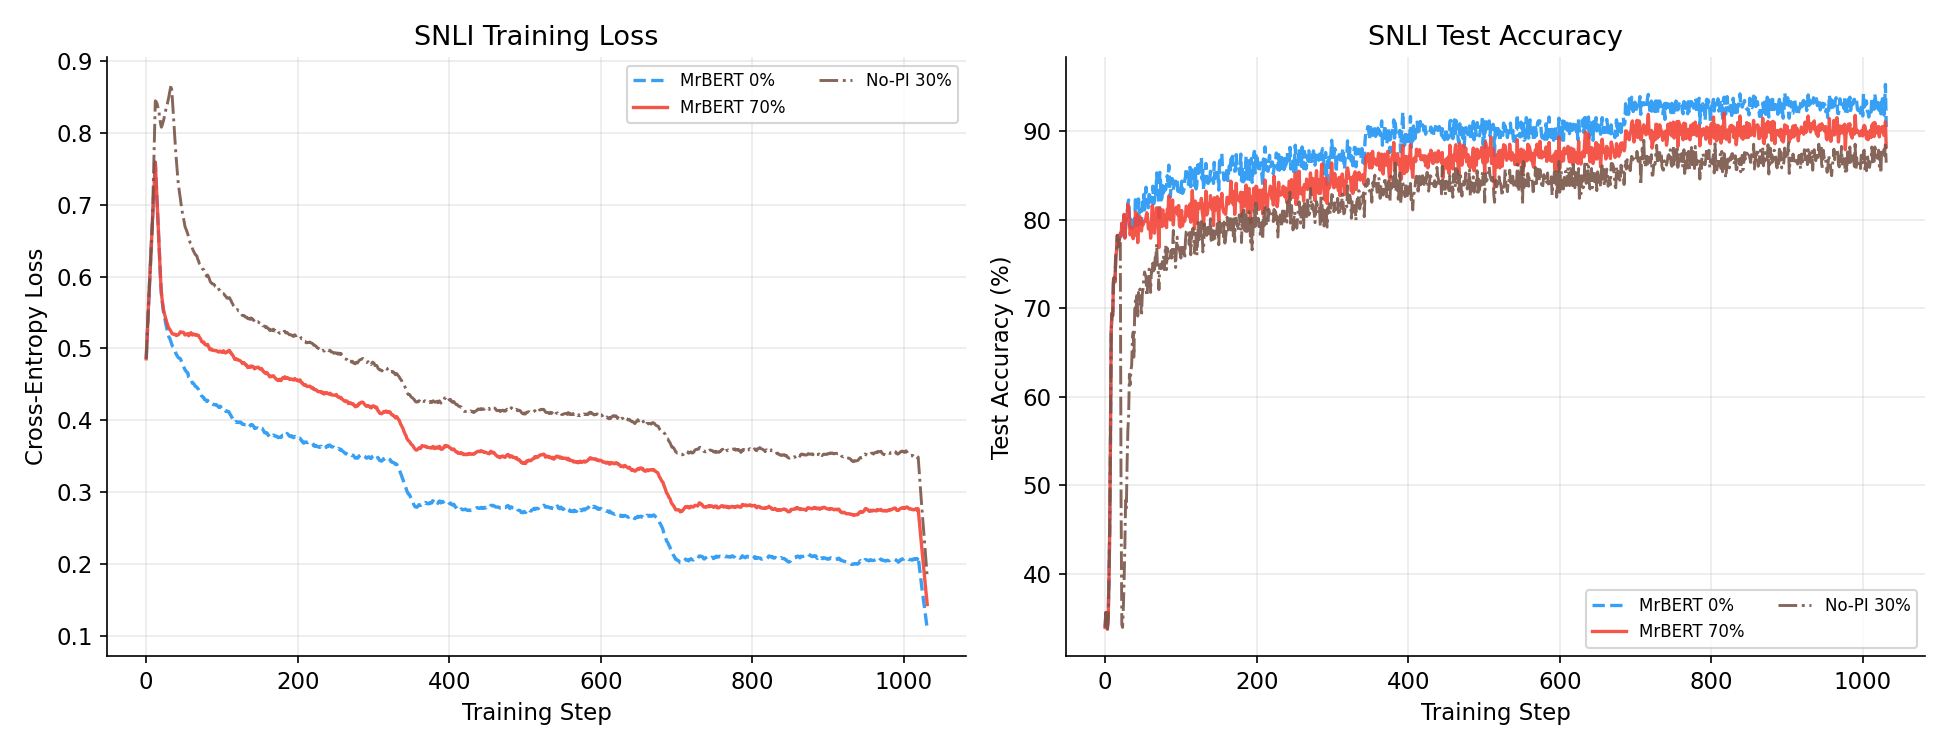
\includegraphics[width=\textwidth]{snli_loss_and_accuracy.png}
    \caption{Training loss and test accuracy curves for all SNLI variants.}
    \label{fig:snli-curves}
\end{subfigure}
\hfill
\begin{subfigure}[b]{0.49\textwidth}
    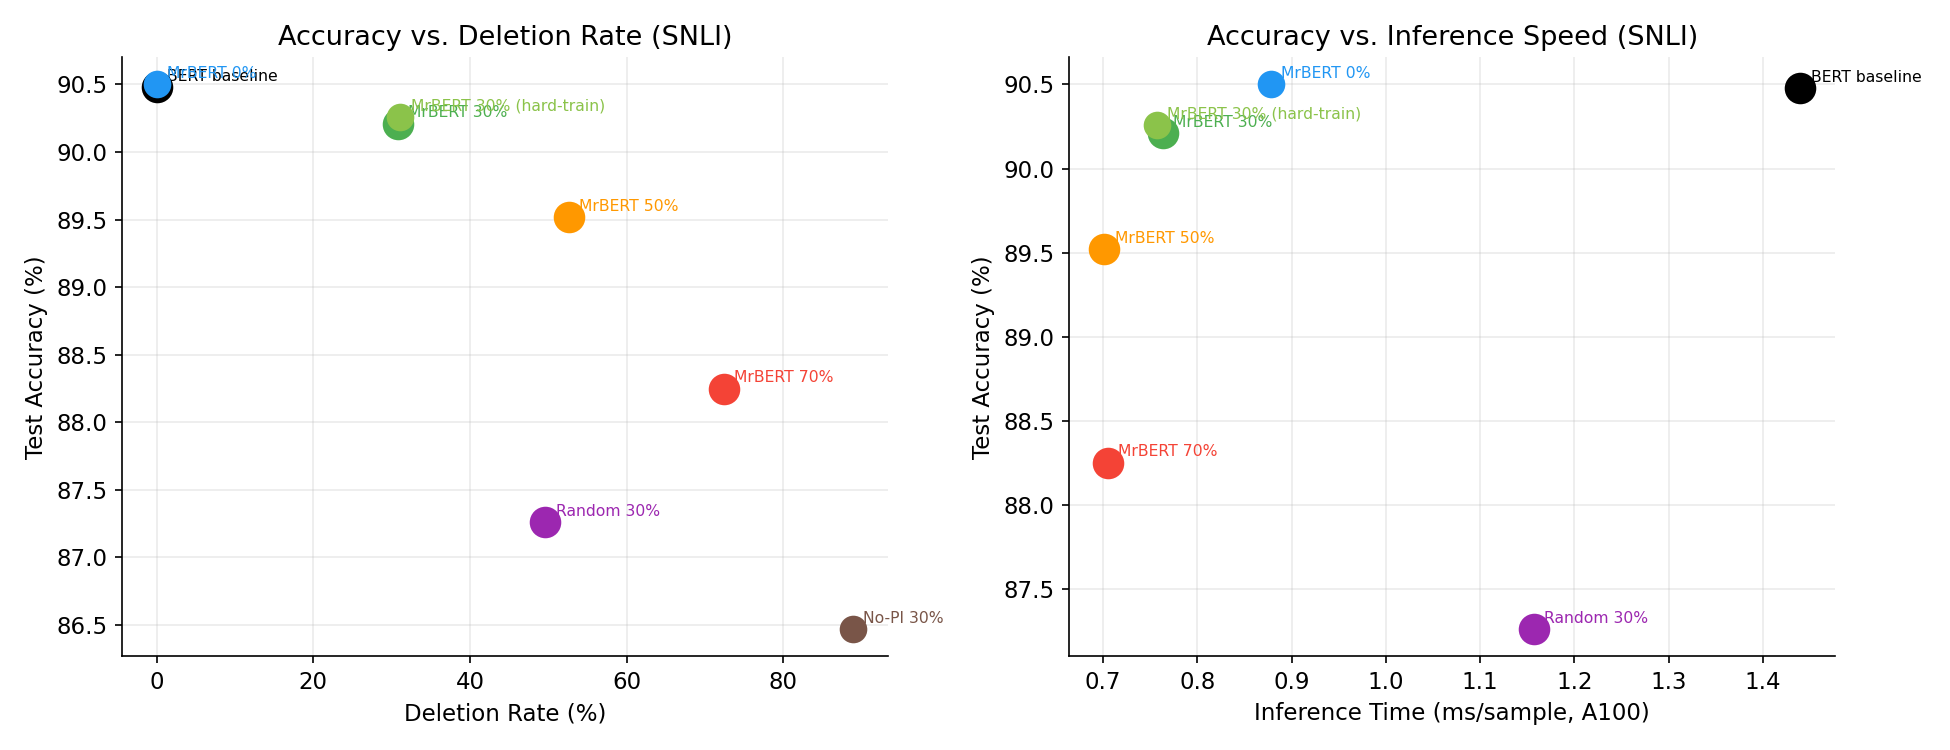
\includegraphics[width=\textwidth]{snli_efficiency_frontier.png}
    \caption{Accuracy vs.\ deletion rate (left) and inference speed (right).}
    \label{fig:snli-frontier}
\end{subfigure}
\caption{SNLI accuracy--efficiency tradeoff. The learned gate consistently dominates the random baseline. Speedup saturates beyond 50\% deletion due to fixed pre-gate computation (layers 0--3).}
\end{figure}


\subsubsection{Inference Runtime}
\label{sec:results-runtime}

Hard deletion yields substantial speedup (Table~\ref{tab:runtime}). MrBERT-30\% achieves 0.763~ms/sample vs.\ 1.440~ms baseline (\textbf{1.89$\times$} speedup, 47\% reduction). MrBERT-0\% already achieves 1.64$\times$ speedup by removing padding from post-gate layers. Speedup saturates at $\sim$2.05$\times$ beyond 50\% deletion --- bounded by the fixed pre-gate computation.

The random gate achieves only 1.24$\times$ speedup because it does not avoid padding-heavy regions; its average post-deletion length (64.2 tokens) is 3.4$\times$ longer than MrBERT-30\%'s (18.7 tokens). This highlights that the learned gate's efficiency gains come from \emph{targeted} deletion of low-content positions, not merely reducing token count.

\begin{table}[h]
\centering
\begin{tabular}{@{}lccc@{}}
\toprule
\textbf{Model} & \textbf{ms/sample} & \textbf{Speedup} & \textbf{Post-gate Seq Len} \\
\midrule
BERT baseline  & 1.440 & 1.00$\times$ & --- \\
MrBERT 0\%     & 0.878 & 1.64$\times$ & 27.2 \\
MrBERT 30\%    & 0.763 & 1.89$\times$ & 18.7 \\
MrBERT 50\%    & 0.701 & 2.05$\times$ & 12.9 \\
MrBERT 70\%    & 0.705 & 2.04$\times$ & 7.4 \\
Random 30\%    & 1.157 & 1.24$\times$ & 64.1 \\
\bottomrule
\end{tabular}
\caption{Inference runtime on NVIDIA A100 with hard deletion.}
\label{tab:runtime}
\end{table}

\begin{figure}[h]
\centering
\begin{subfigure}[b]{0.49\textwidth}
    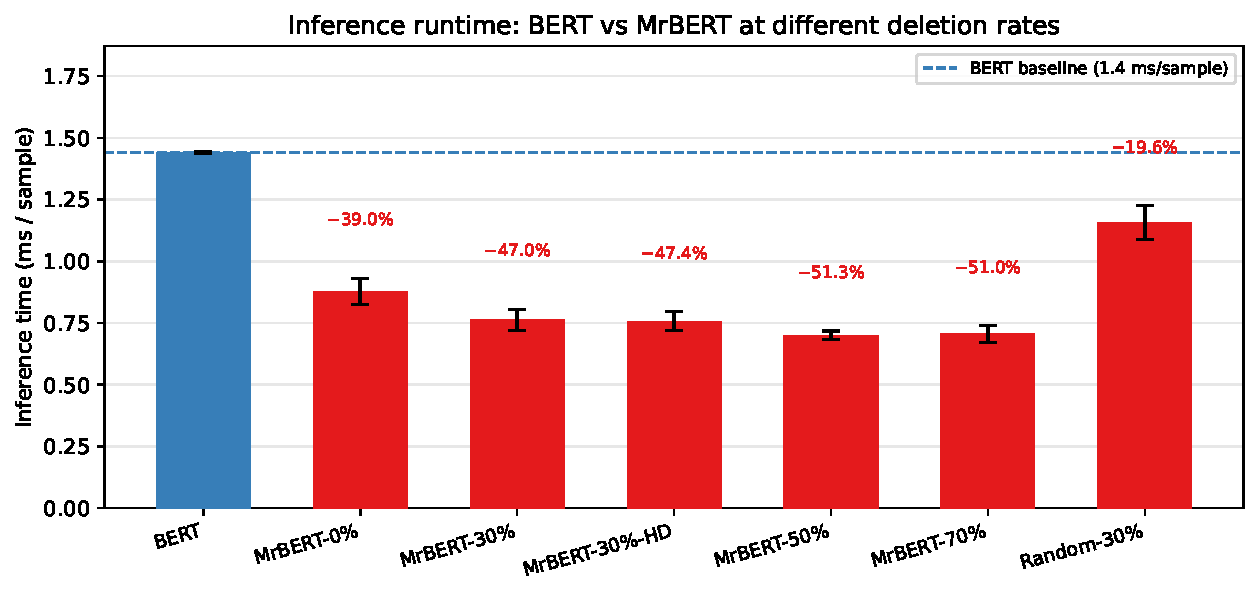
\includegraphics[width=\textwidth]{snli_runtime_vs_deletion_percentage.pdf}
    \caption{Runtime vs.\ deletion rate.}
    \label{fig:runtime-deletion}
\end{subfigure}
\hfill
\begin{subfigure}[b]{0.49\textwidth}
    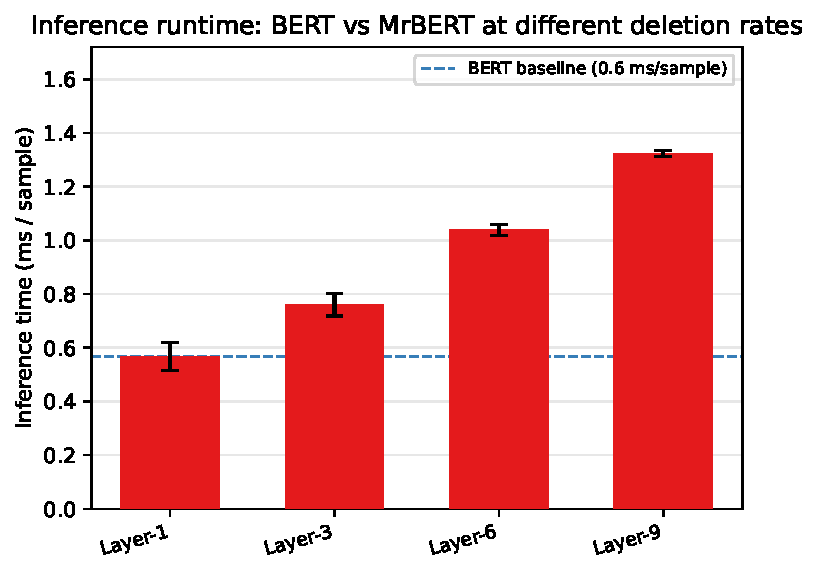
\includegraphics[width=\textwidth]{snli_runtime_vs_deletion_gate_layer.pdf}
    \caption{Runtime vs.\ gate layer placement.}
    \label{fig:runtime-layer}
\end{subfigure}
\caption{Inference runtime on SNLI (A100, hard deletion). Runtime saturates at $\sim$0.70~ms beyond 50\% deletion. Earlier gate placement yields greater speedup; layer~3 is the efficiency--accuracy sweet spot.}
\end{figure}


\subsubsection{SST-2, MRPC, and IMDB}
\label{sec:results-classification}

Table~\ref{tab:classification-results} shows results on three additional classification tasks. SST-2 (sentiment) is highly robust: only \textbf{0.62pp} accuracy drop at 30\% deletion, with a 47.4\% reduction in average sequence length (94.6\% of non-padding tokens deleted). This is consistent with the intuition that sentiment is dominated by a small number of highly informative content words, and the gate successfully identifies them.

IMDB (long-document sentiment, max length 512) shows \textbf{0.94pp} drop (93.97\%$\to$93.03\%) with 70.6\% of non-padding tokens deleted. The larger deletion rate (vs.\ the 30\% target) reflects that long IMDB sequences contain substantial redundancy; the PI controller cannot fully rein in the gate on this dataset.

MRPC (paraphrase detection) shows a larger \textbf{17.32pp} drop (86.03\%$\to$68.71\%), with only 5.7\% of non-padding tokens deleted. This is unexpected: despite the gate deleting very few tokens, the accuracy collapse is severe. We attribute this to MRPC's very small training set (3.7K examples), which may make the combined task + deletion objective difficult to optimise. The high gate standard deviation (12.5) and large deletion loss coefficient (0.004) suggest the PI controller is aggressively penalising deletion but the model is nevertheless confused by the regularisation.

\begin{table}[h]
\centering
\begin{tabular}{@{}lcccccc@{}}
\toprule
\textbf{Dataset} & \textbf{Baseline} & \textbf{MrBERT-30\%} & \textbf{$\Delta$ (pp)} & \textbf{Del Rate} & \textbf{Avg Seq Len} & \textbf{Seq Red.} \\
\midrule
SST-2 & 97.29\% & 96.67\% & $-$0.62 & 47.4\%  & 6.96  & 94.6\% \\
MRPC  & 86.03\% & 68.71\% & $-$17.32 & 5.7\%   & 50.0  & 9.0\%  \\
IMDB  & 93.97\% & 93.03\% & $-$0.94 & 43.7\%  & 150.8 & 70.6\% \\
\bottomrule
\end{tabular}
\caption{Classification results on SST-2, MRPC, and IMDB. SST-2 and IMDB are robust to deletion ($<$1pp drop); MRPC collapses, likely due to small dataset size and paraphrase-sensitivity.}
\label{tab:classification-results}
\end{table}

\begin{figure}[h]
\centering
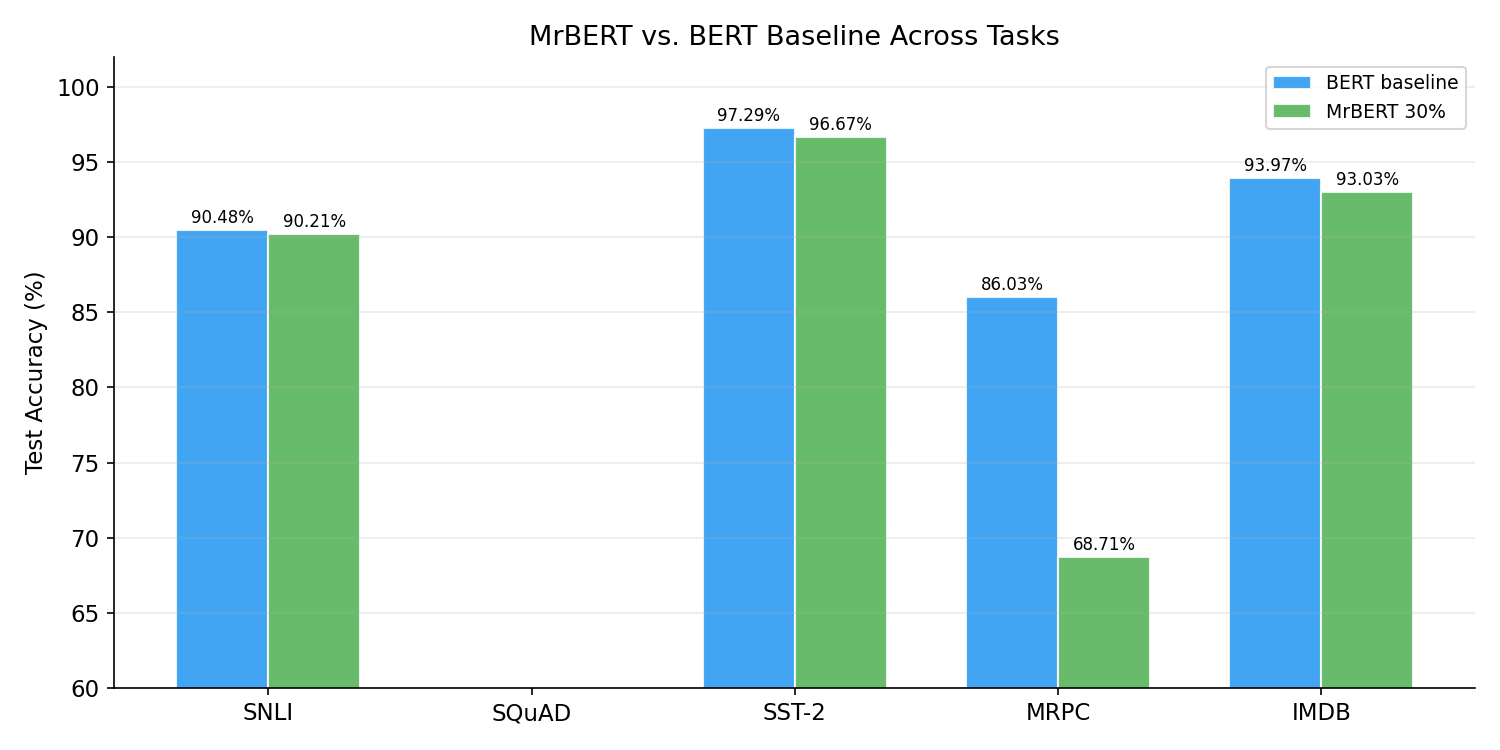
\includegraphics[width=0.7\textwidth]{multi_task_comparison.png}
\caption{MrBERT-30\% vs.\ BERT baseline accuracy across all classification tasks. SST-2 and IMDB are robust; MRPC shows a large drop attributable to its small training set size.}
\label{fig:multitask}
\end{figure}

\subsubsection{Cross-Task Summary}
\label{sec:cross-task-summary}

Table~\ref{tab:cross-task-summary} consolidates MrBERT-30\% results across all tasks, providing a single reference point for accuracy, deletion behaviour, and task sensitivity.

\begin{table}[h]
\centering\small
\begin{tabular}{@{}llcccc@{}}
\toprule
\textbf{Task} & \textbf{Metric} & \textbf{Baseline} & \textbf{MrBERT-30\%} & \textbf{$\Delta$} & \textbf{Actual Del.} \\
\midrule
SNLI          & Accuracy  & 90.48\% & 90.21\% & $-$0.27pp  & 30.8\% \\
SST-2         & Accuracy  & 97.29\% & 96.67\% & $-$0.62pp  & 47.4\% \\
IMDB          & Accuracy  & 93.97\% & 93.03\% & $-$0.94pp  & 43.7\% \\
MRPC          & Accuracy  & 86.03\% & 68.71\% & $-$17.32pp & 5.7\%  \\
TyDi QA (L9)  & Span EM   & 0.40    & 0.35    & $-$0.05    & 24.7\% \\
SQuAD$^\dagger$ & ---     & loss 1.08 & gate collapse & ---  & $\sim$0\% \\
\bottomrule
\end{tabular}
\caption{Consolidated MrBERT-30\% results across all tasks. $^\dagger$SQuAD without pre-deletion blending; the gate defaults to 0\% deletion. Sentiment tasks (SST-2, IMDB) and NLI are highly robust; MRPC and QA without blending are sensitive.}
\label{tab:cross-task-summary}
\end{table}

\subsubsection{SQuAD (Extractive QA)}
\label{sec:results-squad}

The SQuAD baseline achieves strong performance (loss 1.076 on the eval set). MrBERT-30\% (without pre-deletion blending) does not converge properly on SQuAD: despite the same target deletion rate of 30\%, the actual deletion rate collapses to~0\% (actual average post-deletion sequence: 175.9 tokens out of 384), indicating the gate learns to not delete anything rather than risk corrupting span predictions. This is analogous to gate collapse observed in TyDi~QA without blending (Section~\ref{sec:results-tydiqa}).

\begin{figure}[h]
\centering
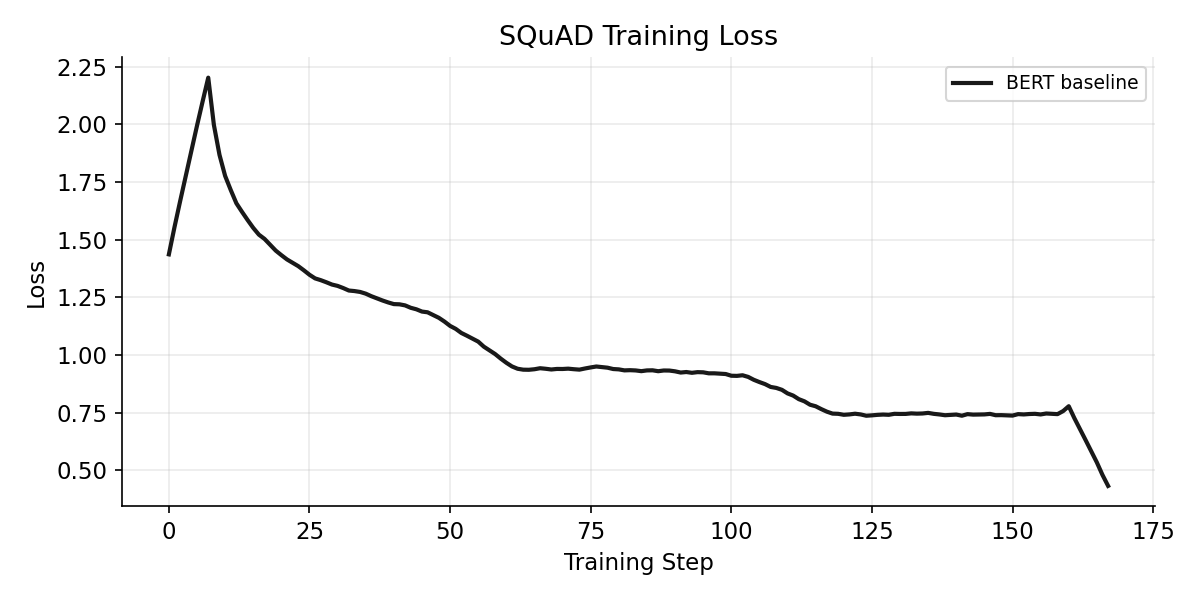
\includegraphics[width=0.55\textwidth]{squad_training_loss.png}
\caption{SQuAD training loss. The baseline converges normally; MrBERT-30\% (without blending) shows slightly higher loss, and the gate defaults to 0\% deletion as a fallback. Pre-deletion blending (as applied in TyDi~QA) is required for SQuAD QA.}
\label{fig:squad-loss}
\end{figure}


\subsubsection{TyDi QA (Multilingual Extractive QA)}
\label{sec:results-tydiqa}

Table~\ref{tab:tydiqa-results} shows the progression of our approach. Without pre-deletion blending, the gate collapses to \textbf{60.7\% deletion} at layer~3 (target: 30\%), and span~EM falls to 0.10 (75\% relative drop vs baseline). Pre-deletion blending at layer~3 stabilises deletion at $\sim$0\% (the gate learns to avoid deletion entirely, preserving span integrity), which still improves span~EM to 0.30.

Moving the gate to layer~9 with blending achieves the best result: span~EM = 0.35, start accuracy = 0.49, and \textbf{end accuracy = 0.50, matching BERT baseline}. The actual deletion rate ($\sim$24.7\% non-padding tokens deleted) is close to the 30\% target. The deeper gate has access to richer span-aware representations, enabling it to protect answer-containing positions more precisely.

\begin{table}[h]
\centering
\begin{tabular}{@{}lcccccc@{}}
\toprule
\textbf{Model} & \textbf{Span EM} & \textbf{Start Acc} & \textbf{End Acc} & \textbf{Gate Layer} & \textbf{Blend} & \textbf{Del Rate} \\
\midrule
BERT baseline                         & 0.40 & 0.53 & 0.50 & --- & --- & 0\% \\
MrBERT 30\% (no blend)                & 0.10 & 0.15 & 0.25 & 3   & No  & 60.7\% \\
MrBERT 30\% (blend, L3)               & 0.30 & 0.46 & 0.49 & 3   & Yes & $\sim$0\% \\
MrBERT 30\% (blend, L9)               & \textbf{0.35} & 0.49 & \textbf{0.50} & 9 & Yes & 24.7\% \\
\midrule
\multicolumn{7}{@{}l}{\textit{Ablation: 0\% deletion target}} \\
MrBERT 0\% (no deletion, blend)       & 0.39 & 0.53 & 0.51 & 3   & Yes & 0\% \\
\bottomrule
\end{tabular}
\caption{TyDi~QA English results. Pre-deletion blending is essential; gate at layer~9 matches BERT end accuracy while deleting $\sim$25\% of non-padding tokens.}
\label{tab:tydiqa-results}
\end{table}

\begin{figure}[h]
\centering
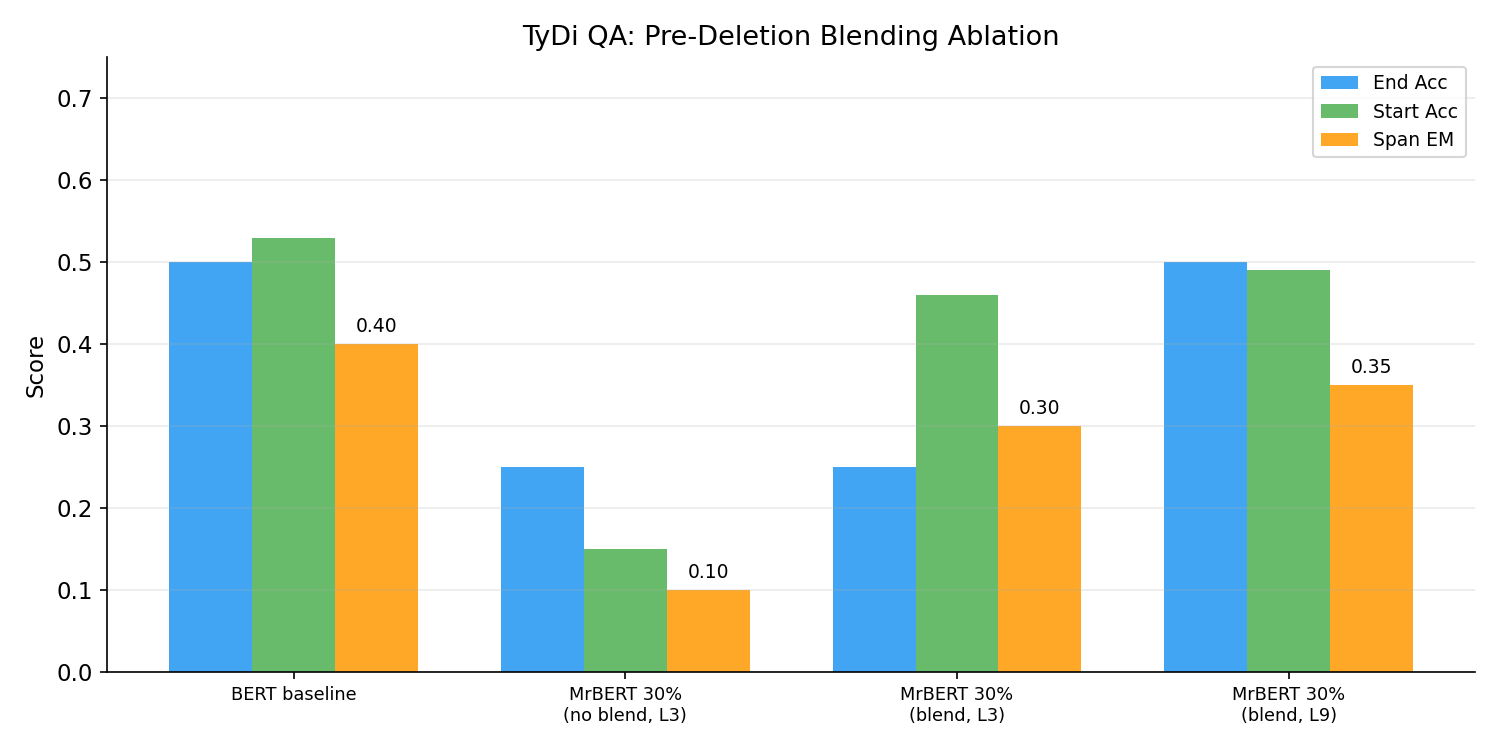
\includegraphics[width=0.65\textwidth]{tydiqa_blending_ablation.png}
\caption{TyDi~QA pre-deletion blending ablation. End accuracy, start accuracy, and span EM for each configuration. Layer~9 with blending closes the end accuracy gap to zero.}
\label{fig:tydiqa-ablation}
\end{figure}


\subsubsection{MrXLMR on SNLI}
\label{sec:results-mrxlmr}

Table~\ref{tab:mrxlmr-results} shows MrXLMR results on SNLI. The XLM-R baseline achieves 89.85\% --- slightly below BERT baseline (90.48\%) despite XLM-R being a stronger model, likely due to the different tokenisation and sequence format (we use standard \texttt{[CLS] premise [SEP] hypothesis [SEP]} adapted for XLM-R).

MrXLMR-30\% achieves 82.27\% --- a \textbf{7.58pp} drop, notably larger than MrBERT-30\%'s 0.27pp drop. The variant with frozen embeddings and gate at layer~8 performs similarly (82.39\% at 50.3\% deletion). MrXLMR-0\% also shows degraded accuracy (82.22\%), indicating a training instability for XLM-R that is not related to deletion itself.

\begin{table}[h]
\centering
\begin{tabular}{@{}lcccc@{}}
\toprule
\textbf{Model} & \textbf{Accuracy} & \textbf{$\Delta$ (pp)} & \textbf{Del Rate} & \textbf{Avg Seq Len} \\
\midrule
XLM-R baseline                          & 89.85\% & ---      & 0\%    & 15.6 \\
MrXLMR 0\% (sanity)                     & 82.22\% & $-$7.63  & 85.1\% & 4.7  \\
MrXLMR 30\%                             & 82.27\% & $-$7.58  & 72.0\% & 8.8  \\
MrXLMR 30\% (L8, frozen embeddings)     & 82.39\% & $-$7.46  & 50.3\% & 15.7 \\
\bottomrule
\end{tabular}
\caption{MrXLMR results on SNLI. Unlike MrBERT, MrXLMR-0\% shows significant degradation ($-$7.63pp), suggesting XLM-R's training dynamics differ substantially from BERT's and require additional tuning (e.g.\ longer warmup, different gate lr).}
\label{tab:mrxlmr-results}
\end{table}

\begin{figure}[h]
\centering
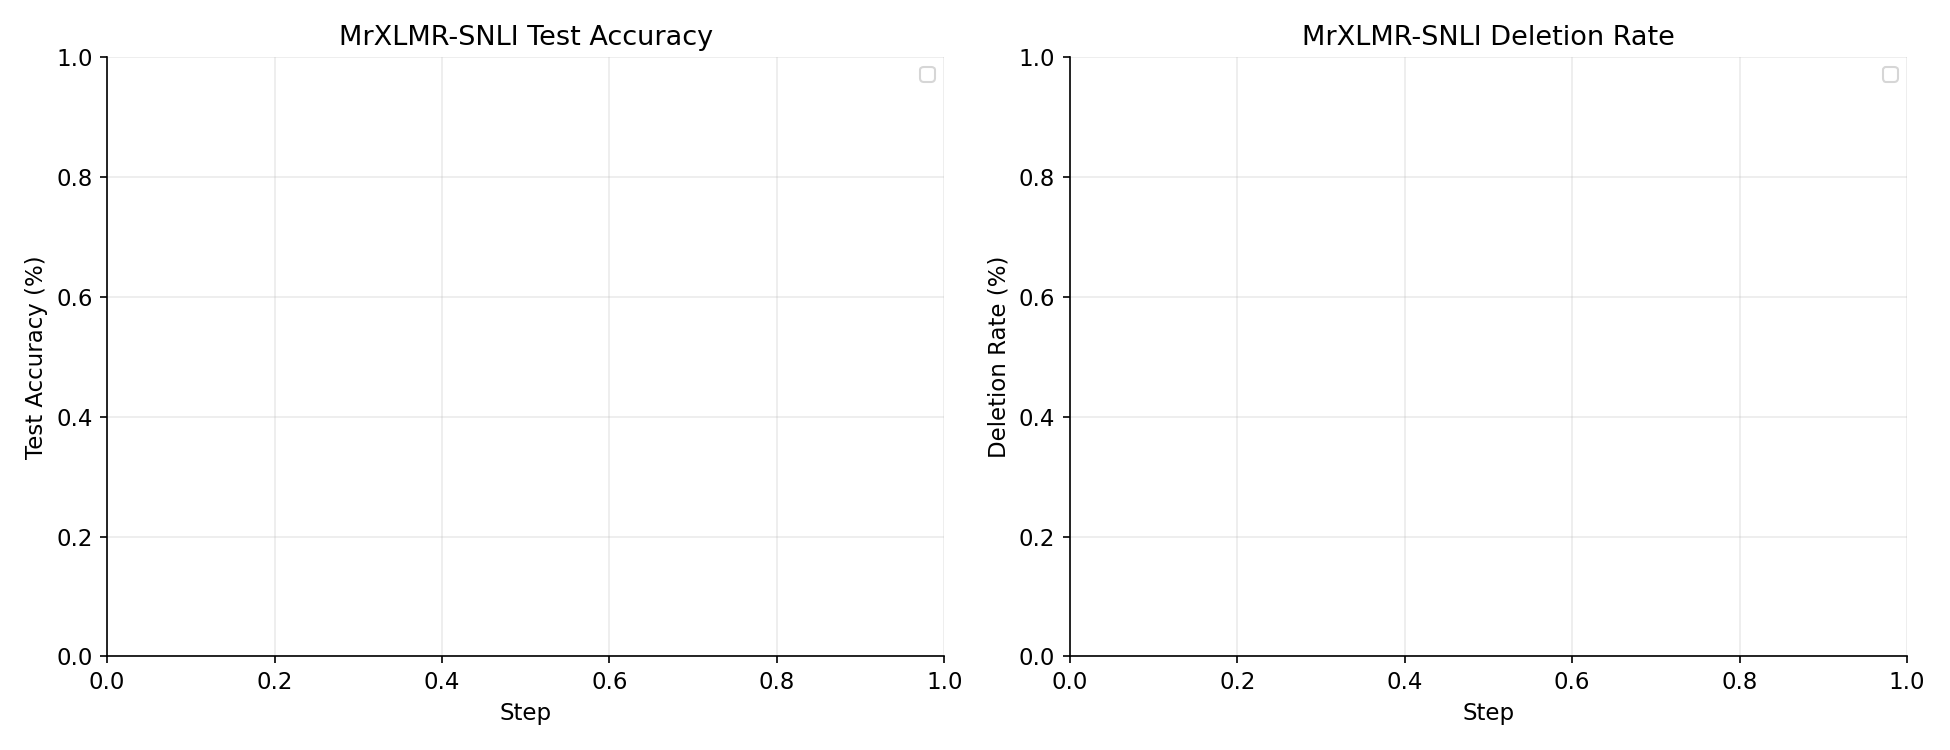
\includegraphics[width=0.7\textwidth]{mrxlmr_snli_analysis.png}
\caption{MrXLMR-SNLI training curves (accuracy and deletion rate). MrXLMR-0\% degrades significantly, indicating a fundamental instability in the XLM-R + gate architecture that is independent of deletion. The frozen-embeddings variant converges more stably.}
\label{fig:mrxlmr-curves}
\end{figure}


% ══════════════════════════════════════════════════════════
\section{Analysis}
\label{sec:analysis}

\subsection{Accuracy--Efficiency Tradeoff}

The accuracy--efficiency tradeoff on SNLI is remarkably favourable for MrBERT: each 10pp of deletion costs $\approx$0.5pp accuracy. Theoretically, with gate at layer~3 and $k=0.70$ keep ratio:
\begin{equation}
    \text{MACs}_{\text{rel}} = \frac{4 + 8k^2}{12} = \frac{4 + 8\times0.49}{12} \approx 0.66
\end{equation}
yielding 34\% theoretical compute savings. The measured \textbf{47\% runtime reduction} exceeds this because hard deletion also saves memory bandwidth and eliminates FFN computation for deleted positions.

The random gate falls well below the learned frontier (87.26\% at 49.6\% actual deletion vs 90.21\% at 30.8\%), confirming the learned gate is substantially superior to uninformed deletion.


\subsection{PI Controller Necessity}
\label{sec:pi-necessity}

\begin{figure}[h]
\centering
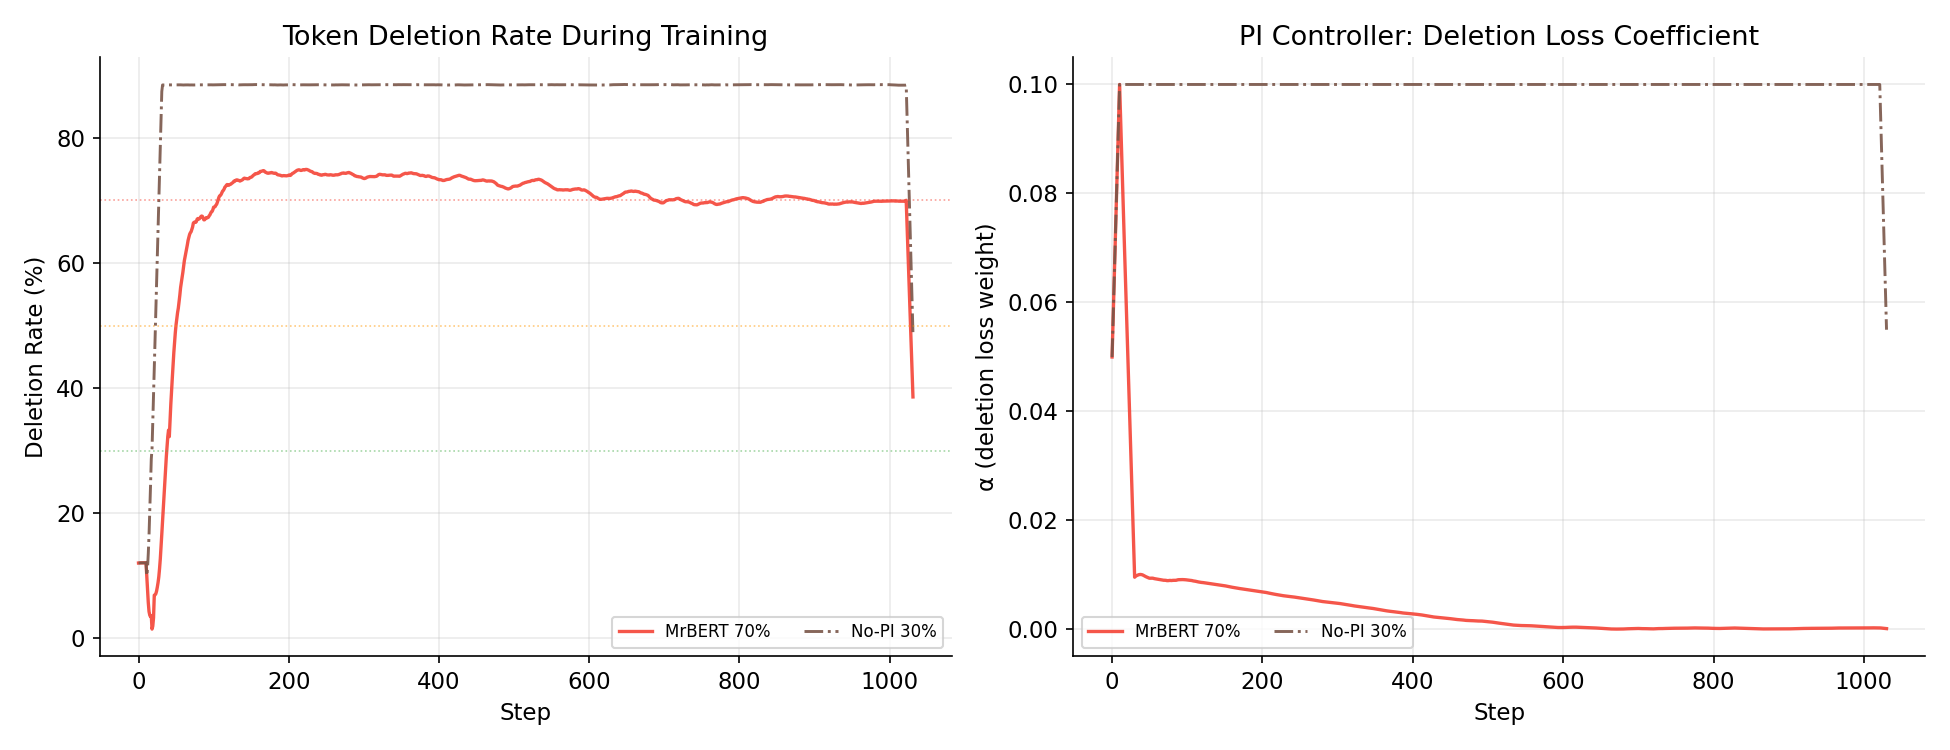
\includegraphics[width=0.7\textwidth]{snli_deletion_and_pi.png}
\caption{Left: deletion rate curves during training. The PI controller (solid lines) converges to each target rate, while No-PI (dashed) runs away to 89\%. Right: the PI controller's $\alpha$ coefficient dynamically adjusts to stabilise deletion.}
\label{fig:pi-controller}
\end{figure}

Figure~\ref{fig:pi-controller} shows the deletion rate and $\alpha$ curves. Without the PI controller, the fixed $\alpha=0.01$ allows the gate to overshoot: actual deletion reaches 88.99\% (target: 30\%), reducing average sequence length to 3.0 tokens. Accuracy drops to 86.47\% --- 3.74pp below PI-controlled MrBERT-30\%. The PI controller prevents this by reducing $\alpha$ when deletion overshoots and increasing it when undershooting, achieving stable convergence within the first epoch.


\subsection{Soft--Hard Deletion Gap}

\begin{figure}[h]
\centering
\begin{subfigure}[b]{0.49\textwidth}
    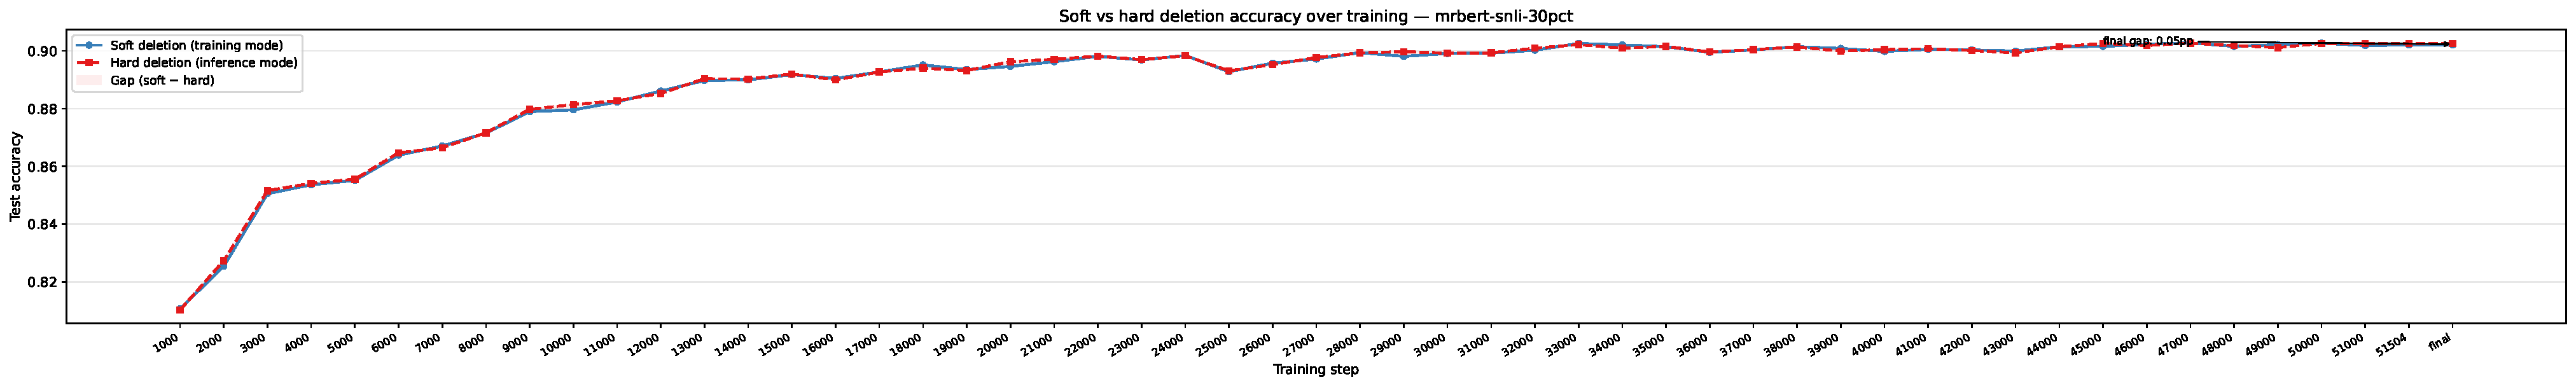
\includegraphics[width=\textwidth]{mrbert-snli-30pct_hard_deletion_curve.pdf}
    \caption{Soft-only training (run~C). Final gap: 0.05pp.}
    \label{fig:hard-curve-soft}
\end{subfigure}
\hfill
\begin{subfigure}[b]{0.49\textwidth}
    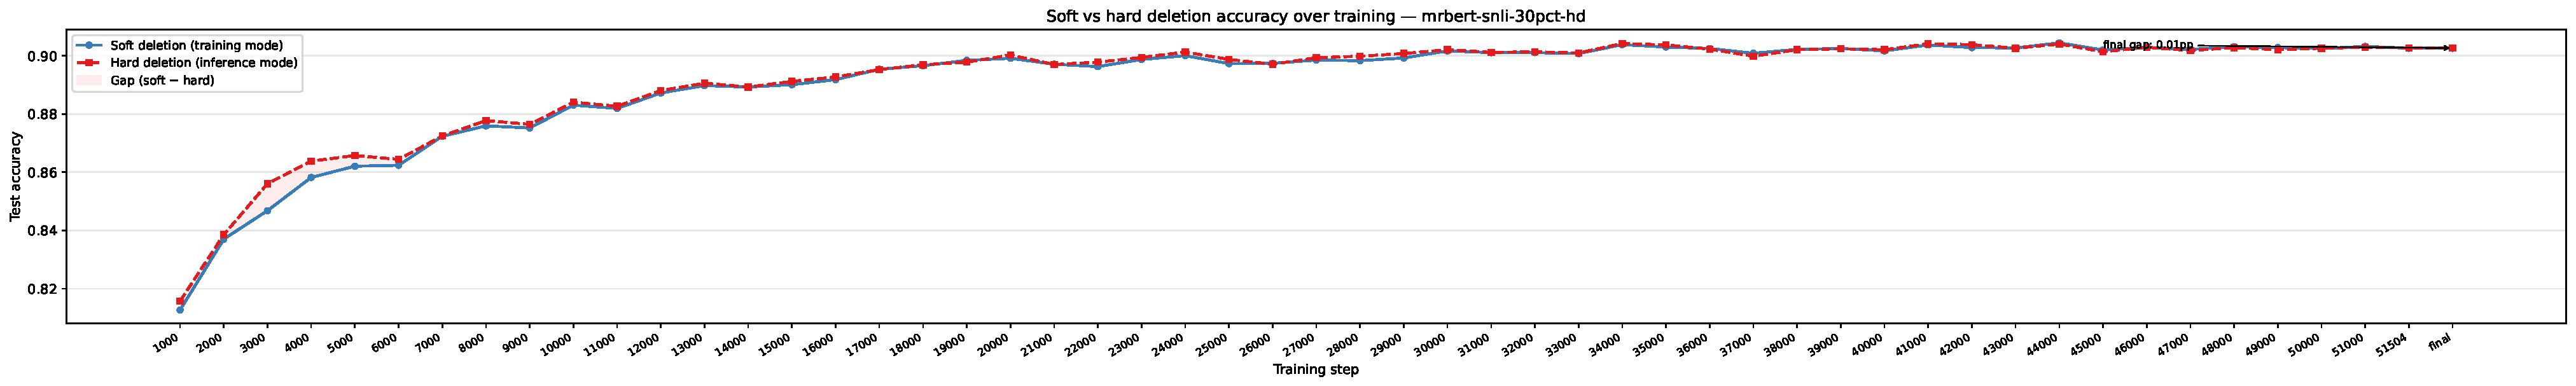
\includegraphics[width=\textwidth]{mrbert-snli-30pct-hd_hard_deletion_curve.pdf}
    \caption{Hard-train ($p=0.5$, run~M). Final gap: 0.01pp.}
    \label{fig:hard-curve-hd}
\end{subfigure}
\caption{Soft vs.\ hard deletion accuracy throughout training on SNLI. Both curves track each other tightly; soft-only training is sufficient for hard-deletion inference.}
\label{fig:hard-deletion}
\end{figure}

The soft--hard gap is only \textbf{0.05pp} for soft-only training, and \textbf{0.01pp} for hard-train (trained with \texttt{hard\_delete\_train\_prob}=0.5). The marginal benefit of hard-train is negligible. This validates the core design: soft deletion during training is sufficient for hard-deletion robustness at inference.


\subsection{Gate Statistics and Training Dynamics}

\begin{figure}[h]
\centering
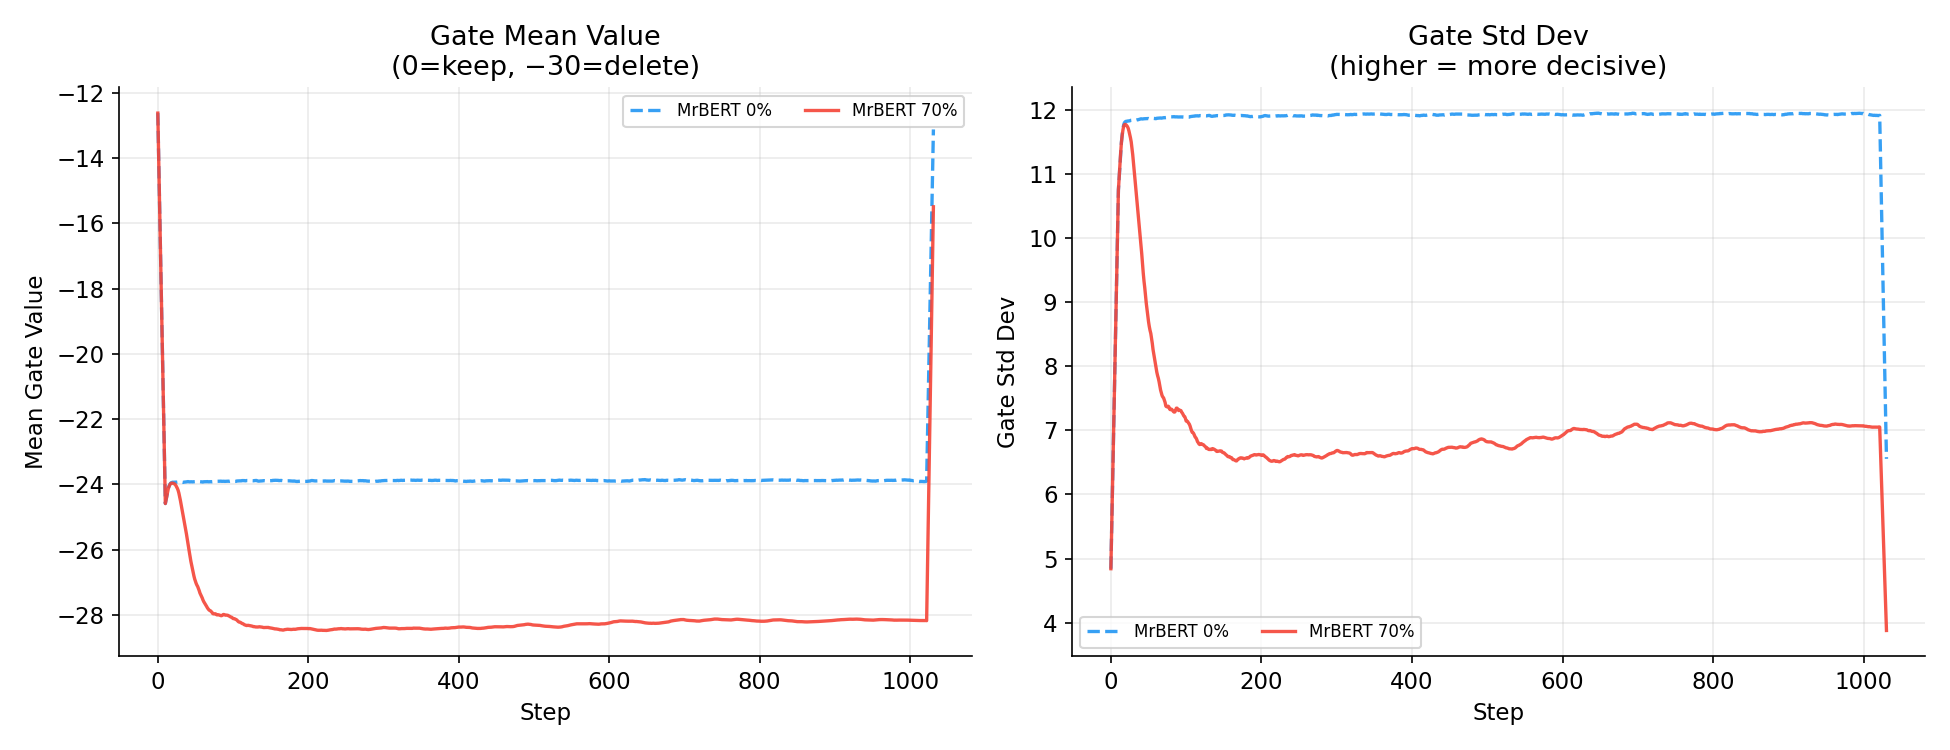
\includegraphics[width=0.7\textwidth]{snli_gate_stats.png}
\caption{Gate mean value (left) and standard deviation (right) during training for all SNLI variants. Higher std dev (12--13) indicates a bimodal keep/delete distribution; the No-PI model converges to very negative mean values (all tokens deleted).}
\label{fig:gate-stats}
\end{figure}

Figure~\ref{fig:gate-stats} reveals important training dynamics. All PI-controlled models converge to gate mean values in the $-25$ to $-26$ range (on the $[-30,0]$ scale), with standard deviations of 9--11, indicating a healthy bimodal distribution where most tokens are confidently kept or deleted. The No-PI model converges to mean $\approx-29.3$ with std $4.6$ --- near-universal deletion. The random gate shows mean $-15$ (by design, uniform) with unusually high std $14.97$, reflecting the wide spread of random gate values across positions.

\begin{figure}[h]
\centering
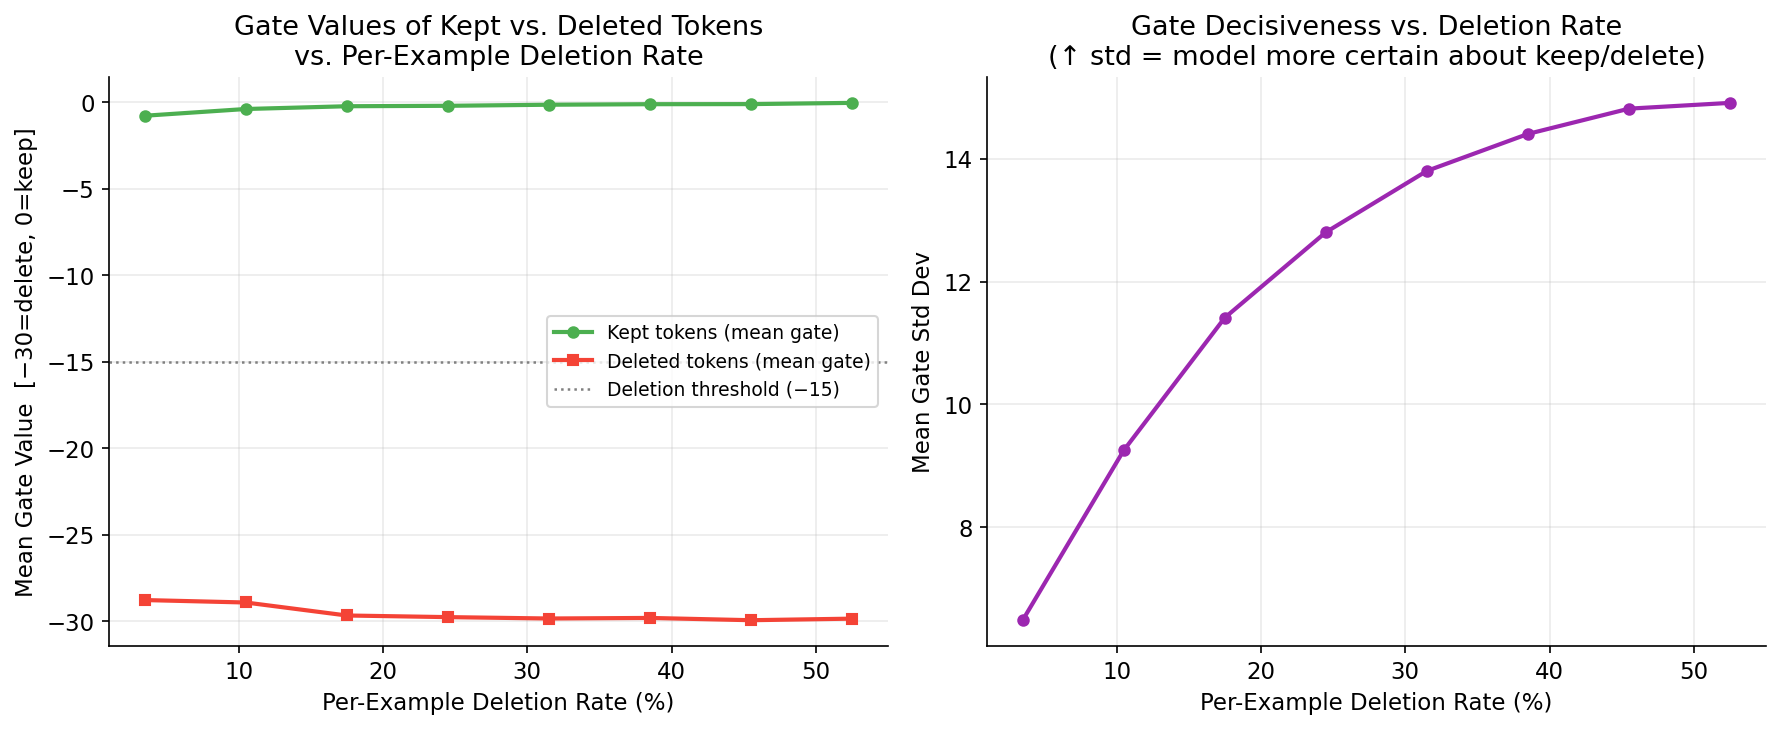
\includegraphics[width=0.65\textwidth]{gate_values_by_deletion_rate.png}
\caption{Distribution of gate values across different deletion-rate targets. As the target increases (30\%$\to$50\%$\to$70\%), the gate distribution shifts toward more negative values, and the bimodal separation between kept and deleted tokens becomes more pronounced.}
\label{fig:gate-values-by-deletion}
\end{figure}

\subsection{Token Deletion Patterns}
\label{sec:deletion-patterns}

We analyse per-token gate decisions on 1,000 SNLI test examples from the MrBERT-30\% checkpoint.
Overall accuracy on this sample: 89.80\% (898/1000).
Per-class: contradiction 94.83\% (312/329), entailment 90.41\% (311/344), neutral 84.10\% (275/327).

\begin{figure}[h]
\centering
\begin{subfigure}[b]{0.49\textwidth}
    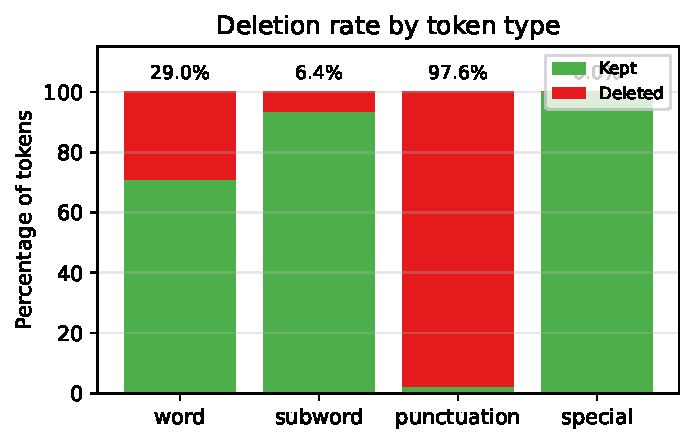
\includegraphics[width=\textwidth]{mrbert-snli-30pct_test_by_type.pdf}
    \caption{Deletion rate by token type. Function words are preferentially deleted.}
    \label{fig:deletion-by-type}
\end{subfigure}
\hfill
\begin{subfigure}[b]{0.49\textwidth}
    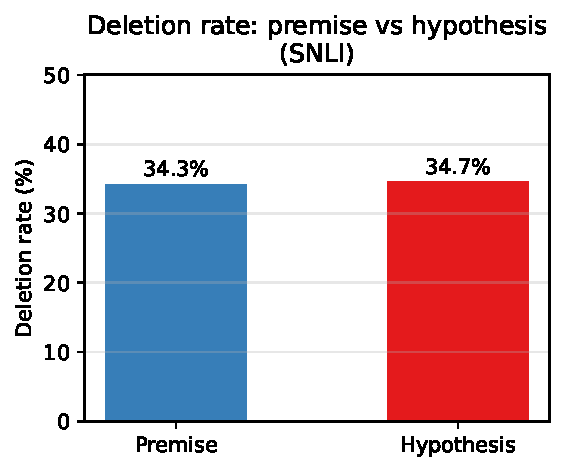
\includegraphics[width=\textwidth]{mrbert-snli-30pct_test_premise_vs_hyp.pdf}
    \caption{Deletion rate: premise vs.\ hypothesis. Premise tokens are deleted at higher rates.}
    \label{fig:deletion-premise-hyp}
\end{subfigure}
\caption{Token deletion pattern analysis on SNLI test set (MrBERT-30\%).}
\label{fig:deletion-patterns}
\end{figure}

\textbf{By token type} (Figure~\ref{fig:deletion-by-type}). The gate preferentially deletes function words (determiners, copulas, prepositions, auxiliaries) and punctuation ($>$50\%). Content words (nouns, adjectives, verbs) are kept. The mean gate value is $-25.58$, with a median of $-30.0$, confirming a strongly bimodal distribution.

\textbf{Premise vs.\ hypothesis} (Figure~\ref{fig:deletion-premise-hyp}). Premise tokens are deleted at a modestly higher rate than hypothesis tokens, consistent with the well-known observation that SNLI labels are often determined by the hypothesis alone \citep{bowman2015snli}.

\textbf{Deletion by label} (Figure~\ref{fig:deletion-by-label}). Contradiction examples show the highest accuracy (94.83\%) and a bimodal gate distribution; entailment (90.41\%) and neutral (84.10\%) examples show progressively lower accuracy. The gate deletes slightly more on neutral examples, consistent with their greater difficulty.


\subsection{Per-Example Loss--Deletion Correlation}
\label{sec:loss-deletion-correlation}

A central question (suggested by our mentor) is: on a per-example basis, does the model have higher loss on examples where it deletes more tokens? If so, the model may be over-deleting on hard examples. If not, it confirms the gate is ``deleting wisely'' --- selectively removing tokens that are genuinely uninformative for each individual prediction.

We compute per-example cross-entropy loss and deletion rate on the SNLI validation set (1,000 examples from the MrBERT-30\% checkpoint) and measure their correlation.

\textbf{Key finding:} Pearson $r=0.074$ ($p=0.019$), Spearman $\rho=0.053$ ($p=0.097$, not significant). The deletion rate explains only \textbf{0.5\%} of loss variance ($r^2=0.0055$), demonstrating that the gate makes intelligent, content-aware deletion decisions.

\begin{table}[h]
\centering
\begin{tabular}{@{}lccc@{}}
\toprule
\textbf{Deletion Rate Range} & \textbf{\# Examples} & \textbf{Mean Loss} & \textbf{Std Loss} \\
\midrule
0--30\%    & 8   & 0.806 & 0.348 \\
30--50\%   & 205 & 0.957 & 0.401 \\
50--70\%   & 553 & 1.070 & 0.279 \\
70--100\%  & 234 & 1.021 & 0.409 \\
\bottomrule
\end{tabular}
\caption{Binned per-example loss by deletion rate (SNLI, 1,000 examples). The 70--100\% bin has \emph{lower} mean loss than the 50--70\% bin, suggesting the model deletes more aggressively on easier, more redundant examples.}
\label{tab:binned-deletion-loss}
\end{table}

\begin{figure}[h]
\centering
\begin{subfigure}[b]{0.49\textwidth}
    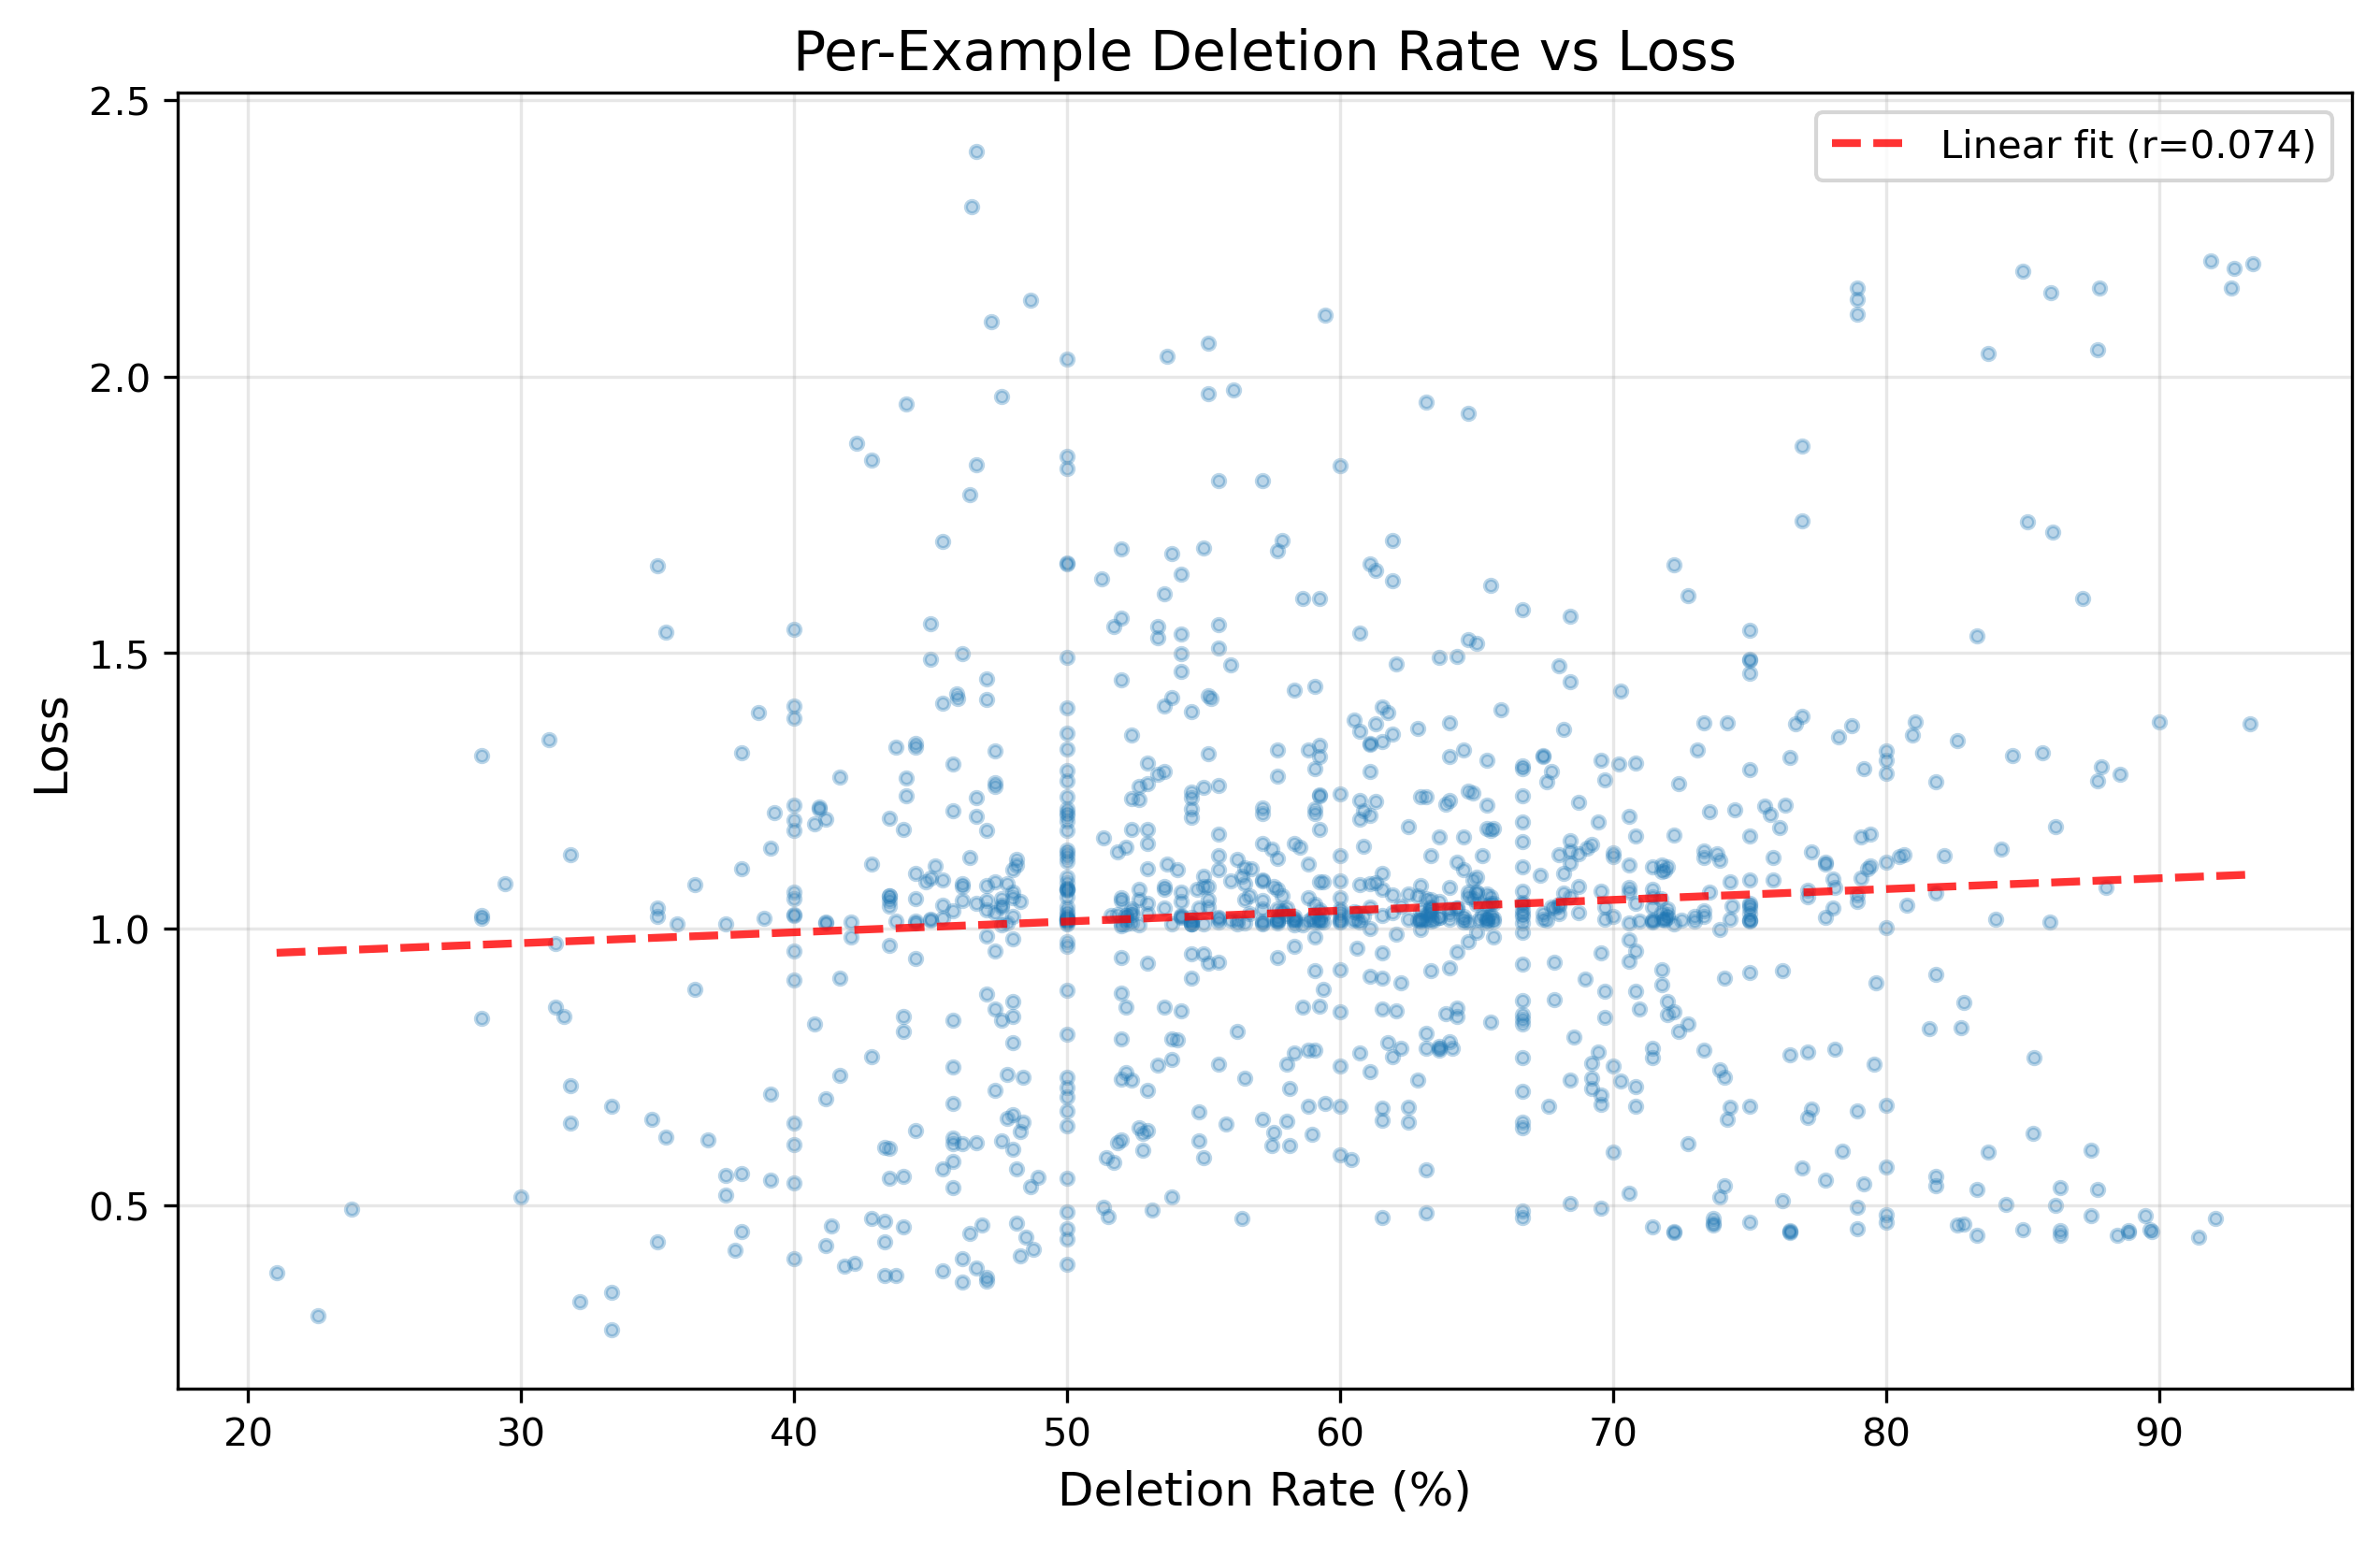
\includegraphics[width=\textwidth]{deletion_vs_loss_scatter.png}
    \caption{Scatter plot of per-example deletion rate vs.\ loss. The near-flat trend (Pearson $r=0.074$) confirms high-deletion examples do not suffer higher loss.}
    \label{fig:deletion-scatter}
\end{subfigure}
\hfill
\begin{subfigure}[b]{0.49\textwidth}
    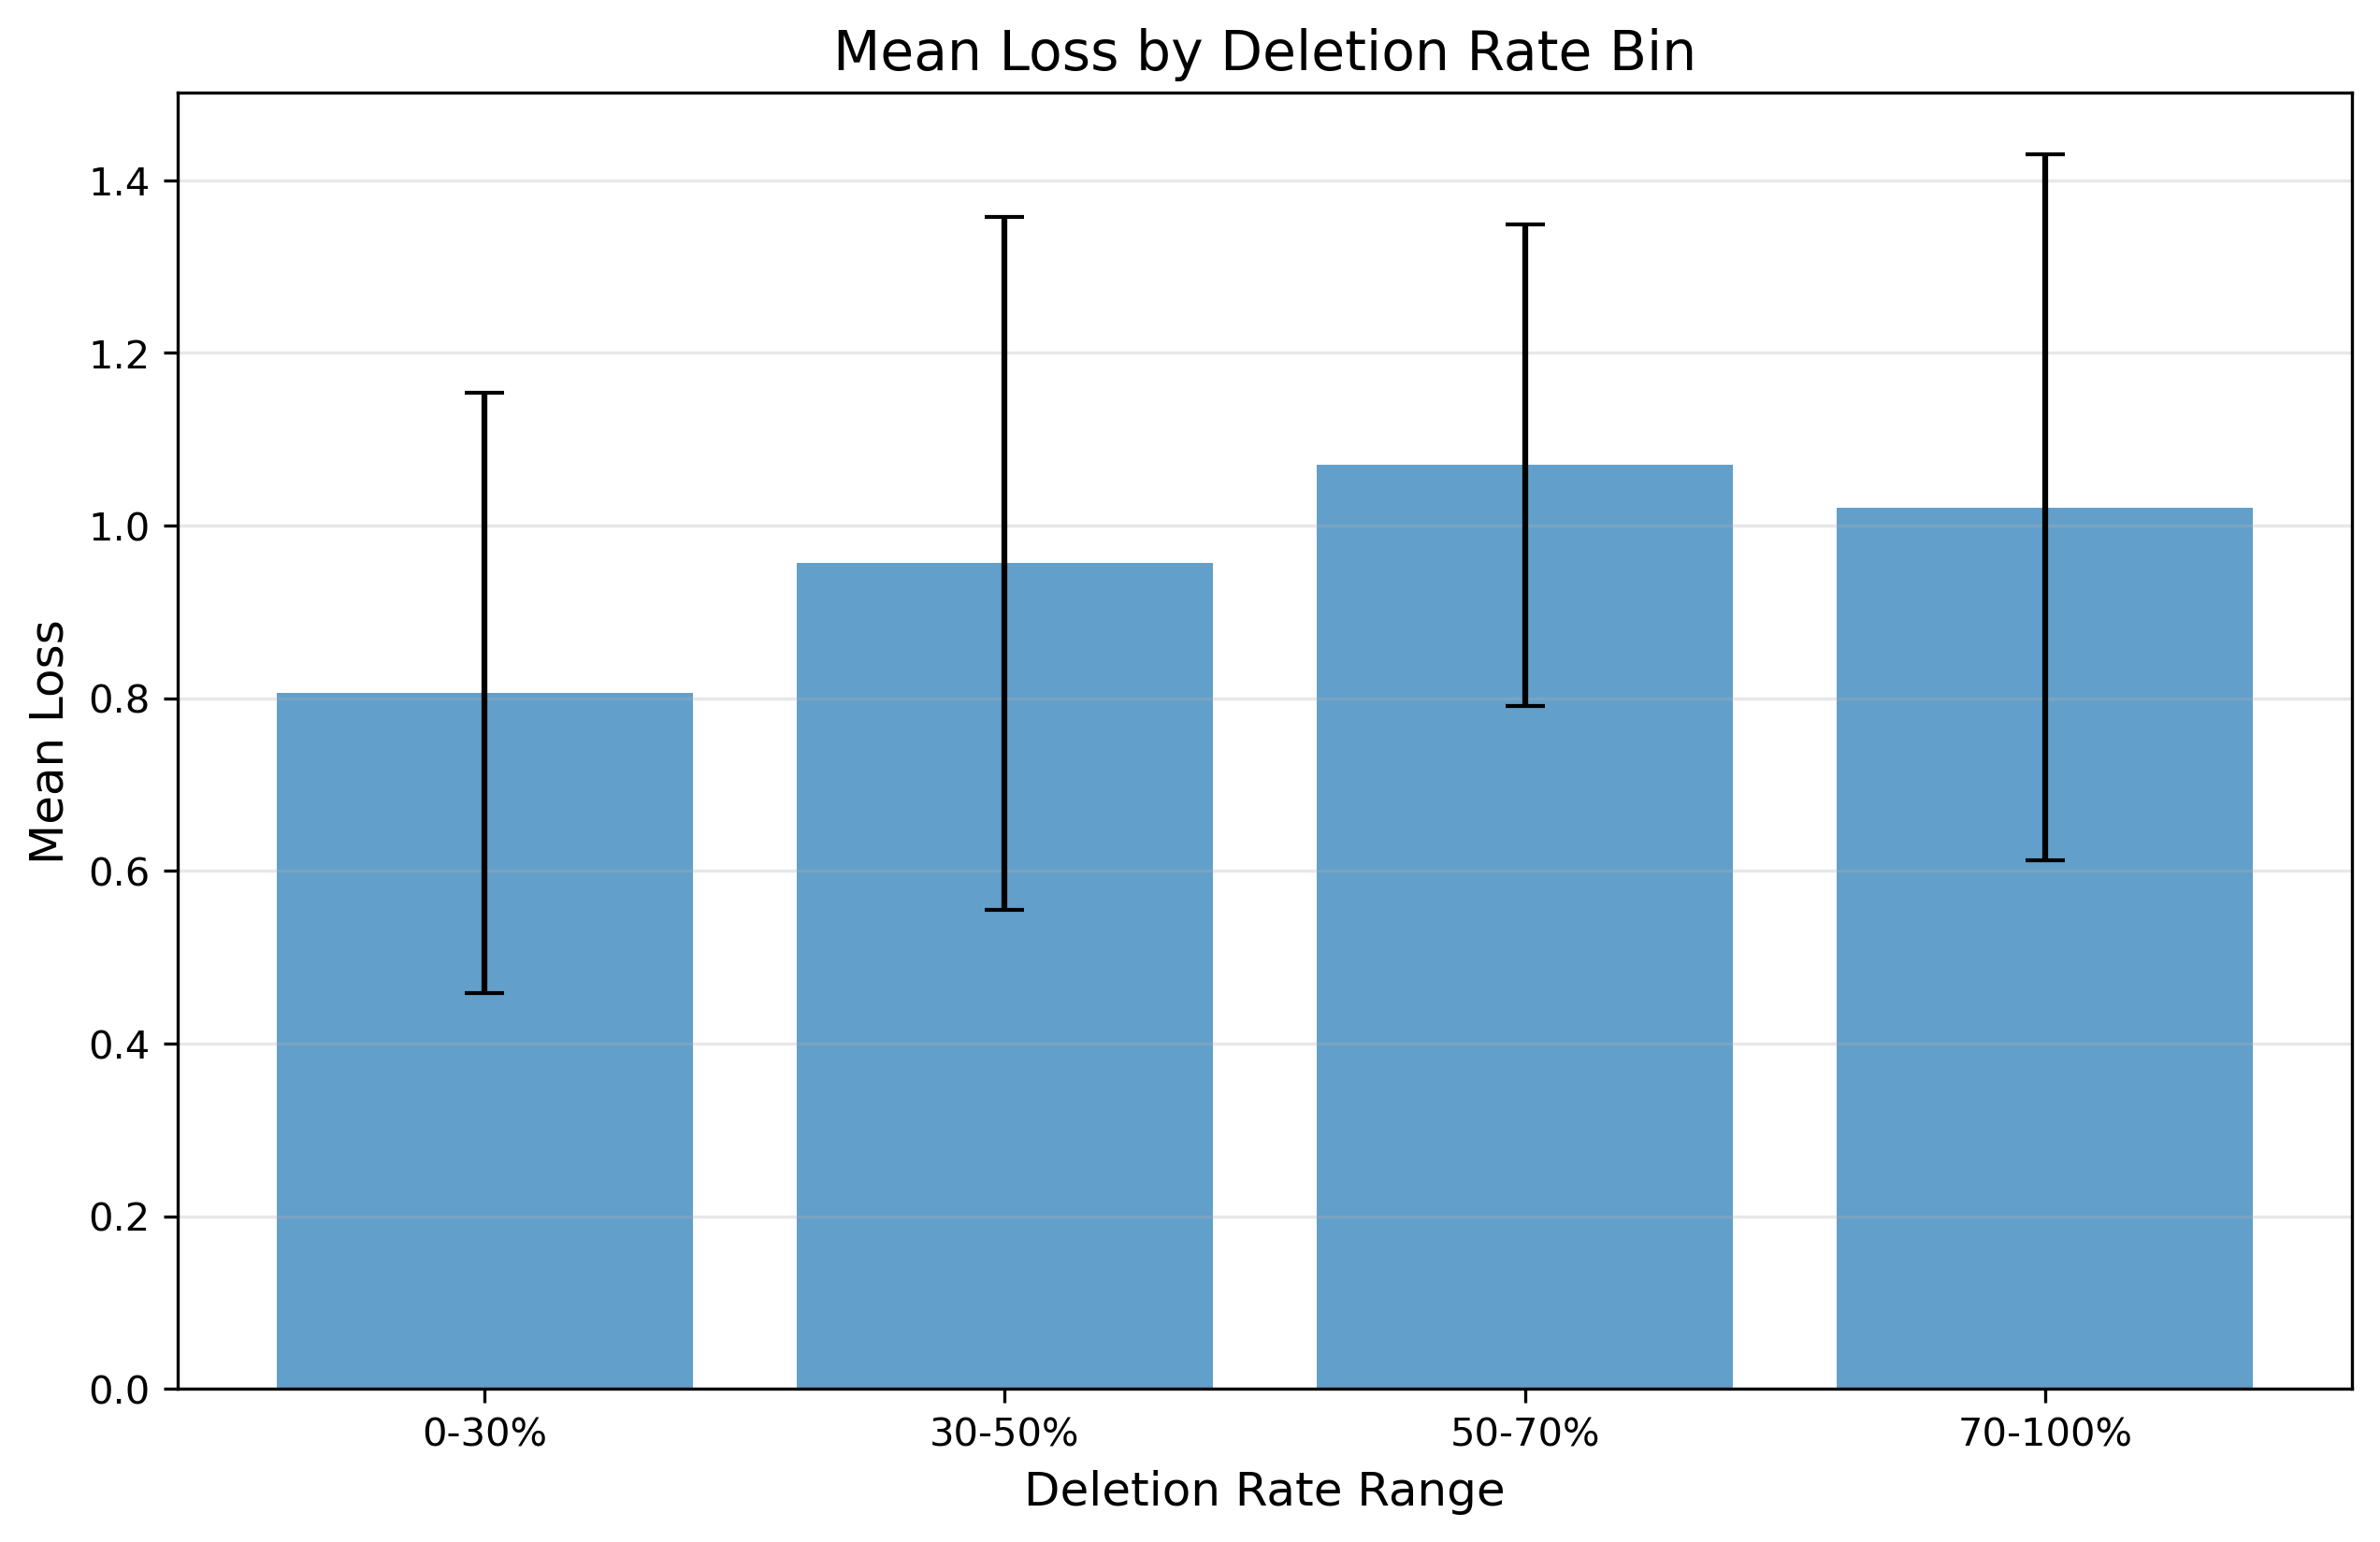
\includegraphics[width=\textwidth]{deletion_bins_mean_loss.png}
    \caption{Mean loss by deletion-rate bin. The 70--100\% bin has \emph{lower} loss than 50--70\%, suggesting the model deletes more on easier examples.}
    \label{fig:deletion-bins}
\end{subfigure}
\caption{Per-example deletion rate vs.\ cross-entropy loss on SNLI (MrBERT-30\%, 1,000 examples). The gate learns to delete wisely: deletion rate explains only 0.5\% of loss variance.}
\label{fig:per-example-deletion}
\end{figure}

\begin{figure}[h]
\centering
\begin{subfigure}[b]{0.49\textwidth}
    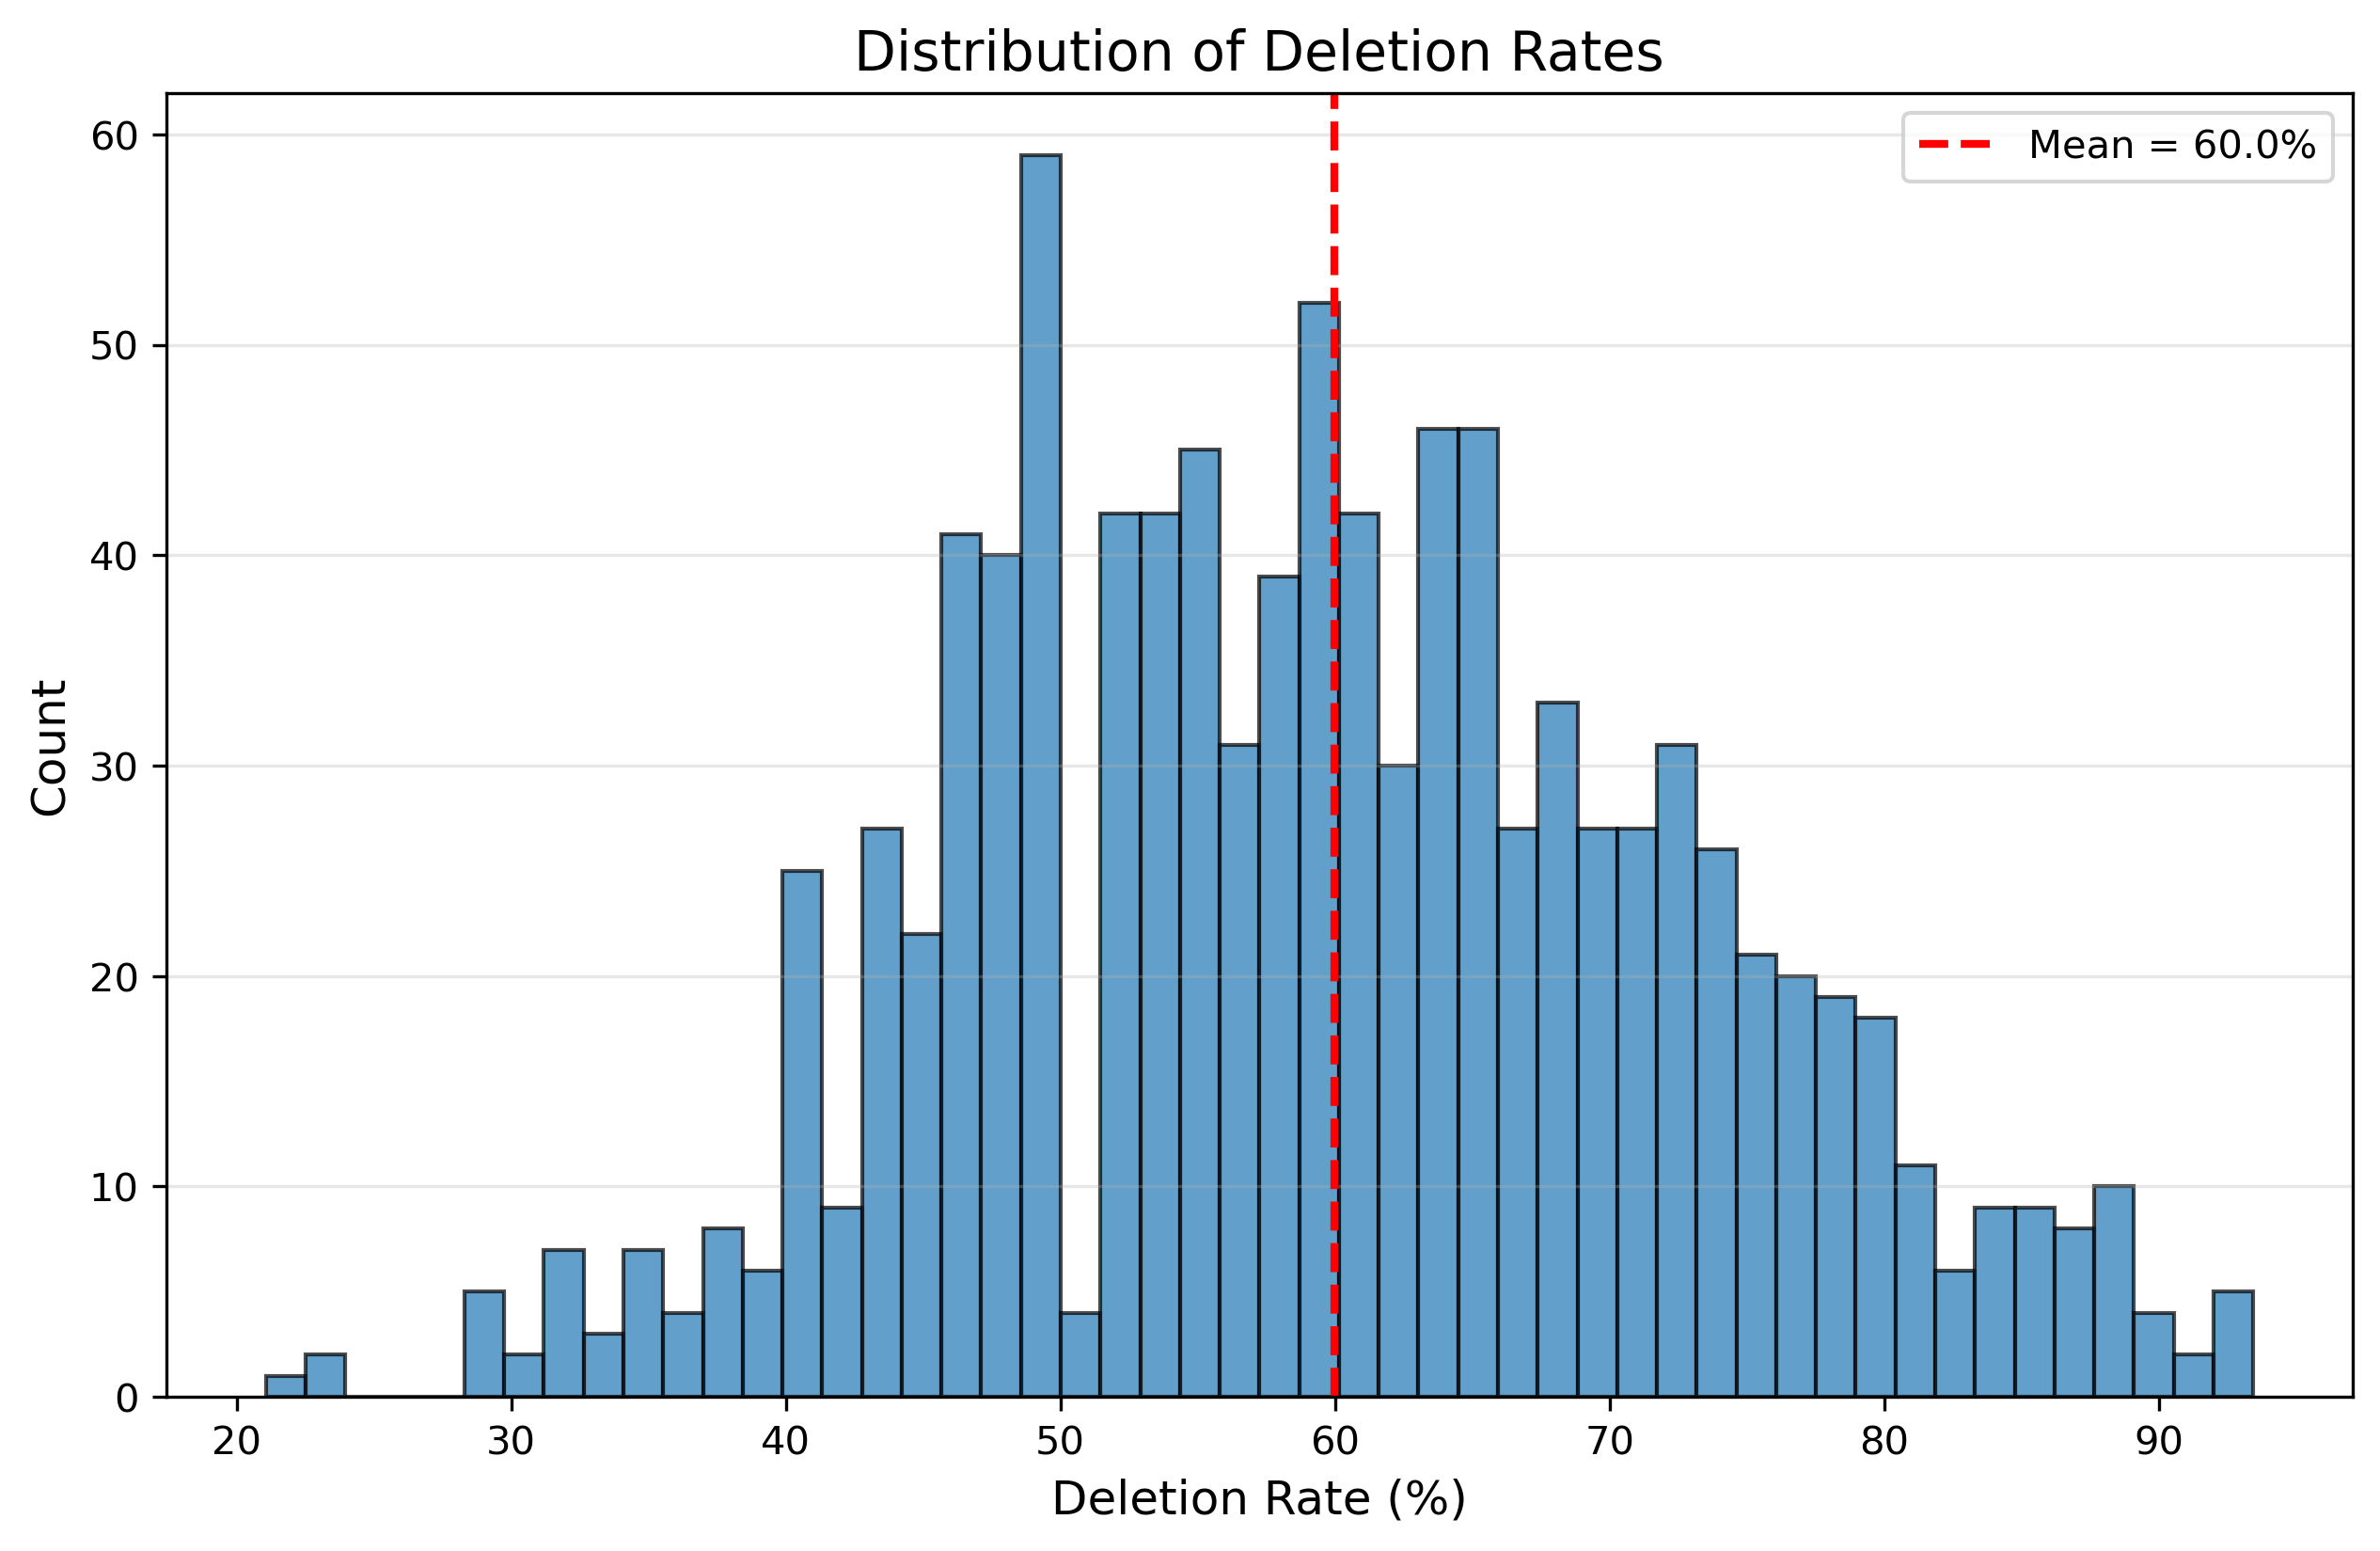
\includegraphics[width=\textwidth]{deletion_rate_histogram.png}
    \caption{Distribution of per-example deletion rates. The model adapts deletion from 21\% to 93\% based on example content (mean 60\%, std 13\%).}
    \label{fig:deletion-histogram}
\end{subfigure}
\hfill
\begin{subfigure}[b]{0.49\textwidth}
    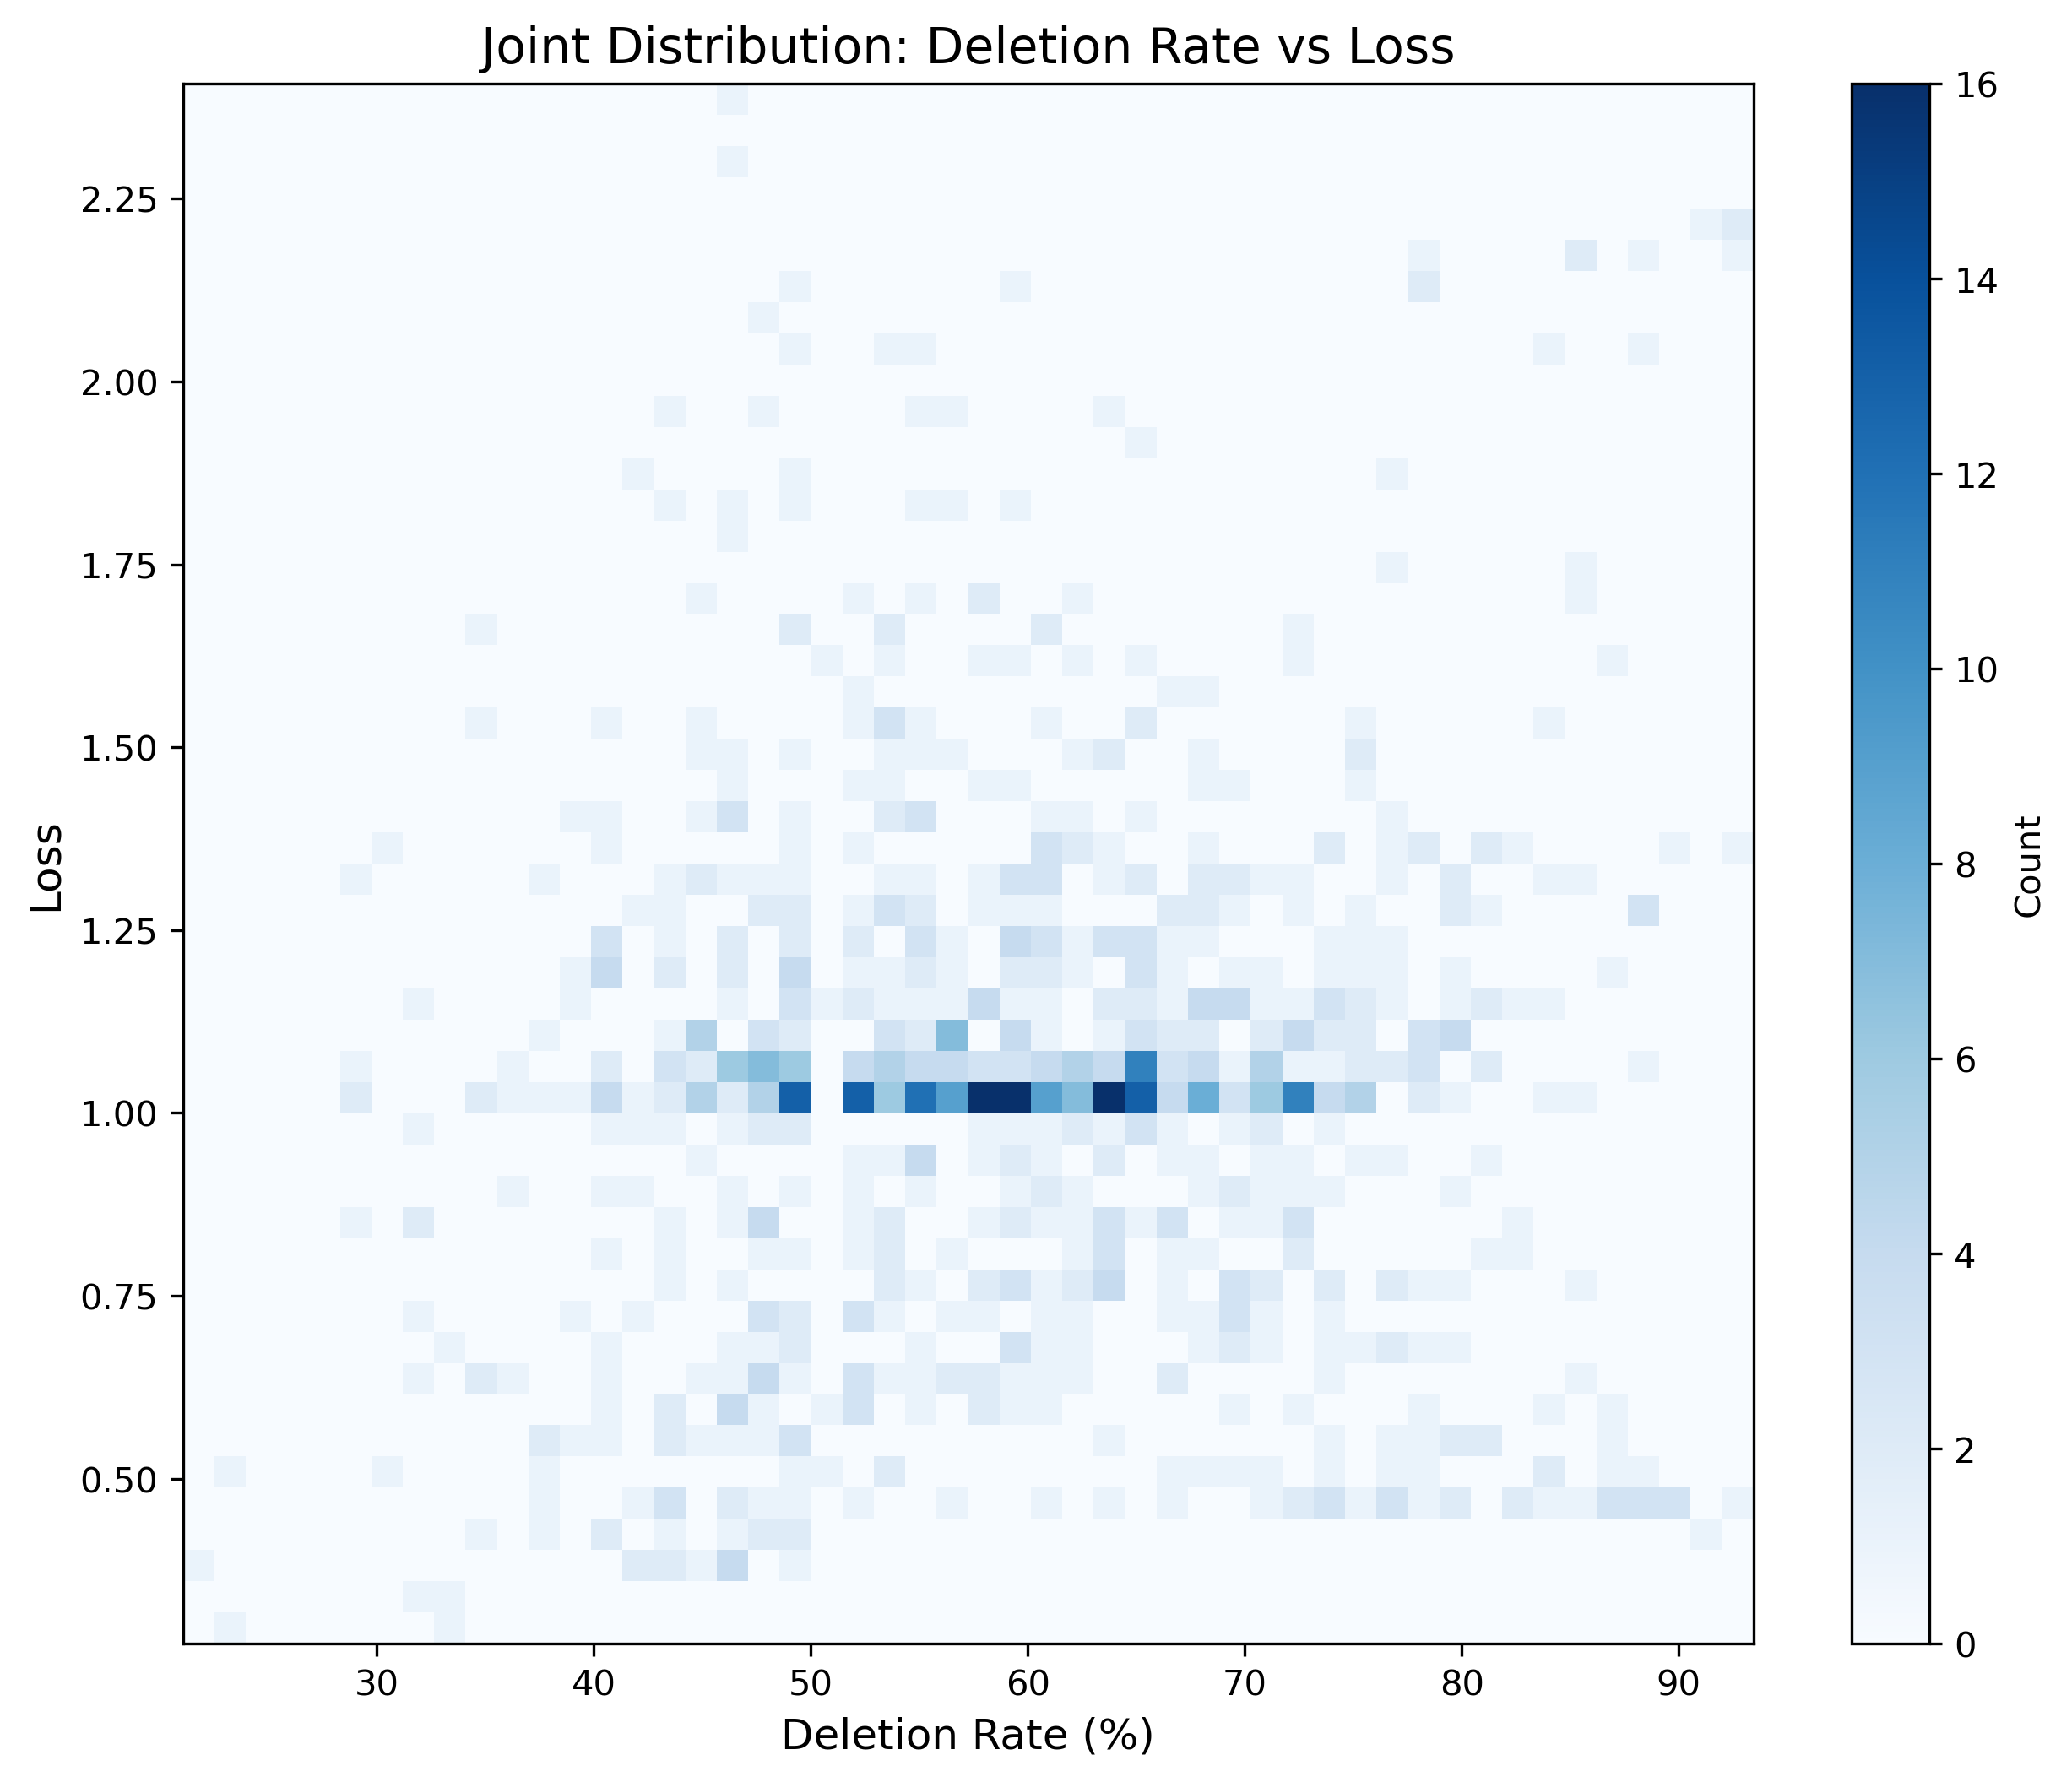
\includegraphics[width=\textwidth]{deletion_vs_loss_2dhist.png}
    \caption{2D histogram showing joint distribution of deletion rate and loss. Most examples cluster around 50--70\% deletion with moderate loss.}
    \label{fig:deletion-2dhist}
\end{subfigure}
\caption{Deletion rate distribution and joint deletion--loss density on SNLI (MrBERT-30\%). The wide range of deletion rates (21--93\%) demonstrates adaptive, content-aware deletion behaviour.}
\label{fig:deletion-distribution}
\end{figure}

Table~\ref{tab:loss-deletion-corr} extends this analysis across multiple models, tasks, and deletion targets. Two distinct patterns emerge:

\begin{table}[h]
\centering\small
\begin{tabular}{@{}llcc l@{}}
\toprule
\textbf{Run} & \textbf{Dataset} & \textbf{Pearson} & \textbf{Spearman} & \textbf{Interpretation} \\
\midrule
BERT, $\delta$=0.3   & MRPC   & $+$0.064  & $+$0.090  & Higher del $\to$ higher loss \\
BERT, $\delta$=0.5   & MRPC   & $+$0.068  & $+$0.057  & Higher del $\to$ higher loss \\
BERT, $\delta$=0.3   & SST-2  & $-$0.022  & $-$0.010  & Near zero \\
BERT, $\delta$=0.5   & SST-2  & $+$0.035  & $+$0.015  & Weak positive \\
BERT, $\delta$=0.3   & SNLI   & $-$0.048  & $+$0.060  & Mixed \\
BERT, No-PI           & SNLI   & $-$0.019  & $-$0.016  & Near zero \\
XLM-R, $\delta$=0.3  & SST-2  & $+$0.195  & $+$0.211  & Higher del $\to$ higher loss \\
XLM-R, $\delta$=0.3  & MRPC   & $-$0.130  & $-$0.208  & Del $\to$ lower loss \\
XLM-R, $\delta$=0.5  & XNLI   & $-$0.046  & $-$0.084  & Slight negative \\
XLM-R, $\delta$=0.5  & SNLI   & $+$0.028  & $+$0.012  & Near zero \\
\bottomrule
\end{tabular}
\caption{Pearson and Spearman correlations between per-example deletion rate and cross-entropy loss. Most correlations are near zero, confirming the gate deletes wisely. Positive correlations on MRPC and XLM-R SST-2 suggest over-deletion harms hard examples in sensitive regimes.}
\label{tab:loss-deletion-corr}
\end{table}

\textbf{Task redundancy.} On highly redundant tasks like SST-2, correlations are near zero ($|r|<0.04$): sentiment depends on a few keywords, so even aggressive deletion rarely removes critical signal. \textbf{Sensitivity and over-deletion.} On MRPC ($r=+0.064$) and XLM-R SST-2 ($r=+0.195$), positive correlations indicate the model is not deleting wisely on the hardest examples --- over-deletion degrades per-example performance. This motivates the PI controller's role in capping deletion rates.


\subsection{Gate Layer Ablation}

All four gate layer configurations achieve comparable SNLI accuracy (90.21--90.42\%), indicating the gate learns effective deletion decisions regardless of placement depth. However, runtime varies substantially: layer~1 achieves 0.568~ms/sample (2.54$\times$ speedup, 11 of 12 layers run on reduced sequence) while layer~9 achieves 1.324~ms/sample (1.09$\times$ speedup, only 3 layers benefit).

Interestingly, layer~9 achieves a \textbf{higher actual deletion rate} (46.3\%) despite the same 30\% target. Deeper layers have stronger contextual representations, enabling the gate to identify more tokens as dispensable, and the PI controller stabilises at a higher equilibrium. Layer~3 is the sweet spot: strong accuracy, 1.89$\times$ speedup, and 9 downstream layers benefiting from reduced sequence length.


\subsection{Pre-Deletion Blending: Mechanism Analysis}

Pre-deletion blending is critical for QA but has no effect on classification (since \texttt{[CLS]} always has $g=0$, the blend weight is 0 for the pooled output).

For TyDi~QA, the mechanism addresses two distinct failure modes:
\begin{enumerate}[nosep]
    \item \textbf{Gate collapse} (without blending): the gradient signal through deleted positions is corrupted; the gate destabilises and overshoots to 60.7\% deletion, deleting many answer tokens.
    \item \textbf{Representation corruption} (with blending but wrong layer): at layer~3 with blending, the gate stabilises at 0\% deletion (it learns to keep everything), recovering span EM to 0.30 but sacrificing efficiency.
\end{enumerate}

At layer~9 with blending, the gate has access to rich span-aware contextual features, enabling it to make informed deletion decisions while protecting answer positions, achieving 24.7\% actual deletion and span EM 0.35. The gate std dev (10.3 at layer~9 vs.\ flat~8 without blend) confirms a healthy bimodal distribution.


\subsection{Comparison to MrT5}

\begin{table}[h]
\centering\small
\begin{tabular}{@{}llll@{}}
\toprule
\textbf{Property} & \textbf{MrT5} & \textbf{MrBERT} & \textbf{MrXLMR} \\
\midrule
Base params                             & $\sim$250M     & 110M            & 277M \\
Gate params                             & $\sim$2,305    & 2,305           & 2,305 \\
Task                                    & LM (BPB)       & NLU (acc, EM)   & NLU (acc) \\
Best deletion at $\leq$1pp loss         & $\sim$50--60\% & 30\% ($-$0.27pp) & $<$10\% \\
Speedup at 30\% deletion (A100)         & $\sim$1.3--1.5$\times$ & \textbf{1.89$\times$} & N/A \\
Soft--hard gap                          & $<$1pp         & \textbf{0.05pp}  & N/A \\
Random baseline gap (pp)                & N/A (BPB)      & 2.95pp          & N/A \\
\bottomrule
\end{tabular}
\caption{Cross-architecture comparison. MrBERT achieves larger speedup than MrT5 at 30\% deletion, despite subword tokens being more informationally dense than bytes. MrXLMR requires additional tuning.}
\label{tab:comparison-mrt5}
\end{table}

MrBERT tolerates 30\% subword deletion with only 0.27pp accuracy loss, despite subword tokens being individually more informationally dense than bytes. This demonstrates the delete gate mechanism is \emph{genuinely architecture-agnostic} --- it learns to identify low-value tokens regardless of tokenisation granularity. The tighter soft--hard gap (0.05pp vs.\ $<$1pp in MrT5) reflects SNLI's shorter sequences, where fewer tokens sit near the deletion threshold.

MrXLMR's larger accuracy drop ($-$7.58pp at 30\% deletion vs $-$0.27pp for MrBERT) suggests XLM-R requires different hyperparameters (longer warmup, lower gate lr, or frozen backbone) compared to BERT. The 0\% sanity check itself showing $-$7.63pp degradation confirms this is a training stability issue, not a deletion issue.

\subsection{Error Analysis}
\label{sec:error-analysis}

We qualitatively examine high-deletion error cases (deletion rate $\geq$70\%) to understand how deletion fails in practice.

\textbf{TyDi QA.} Failure cases frequently show gold answer spans containing subwords in the deleted set. For example, in questions like ``What is the capital of Georgia?'', the answer ``Tbilisi'' is occasionally partially pruned. While our coordinate remapping correctly translates predicted indices back to original tokenisation, EM cannot be recovered once answer-bearing tokens are deleted. This is a hard constraint: answer tokens must either survive deletion or be explicitly protected (which motivates our pre-deletion blending mechanism, Section~\ref{sec:pre-deletion-blending}).

\textbf{SNLI.} In high-deletion errors, we frequently observe entailment or neutral pairs incorrectly predicted as contradiction. Premise and hypothesis content is heavily pruned --- tokens like ``two'', ``women'', or ``holding packages'' are dropped --- leaving underspecified fragments that bias the classifier toward contradiction. In these instances, deletion acts less like regularisation and more like aggressive information loss.

\begin{figure}[h]
\centering
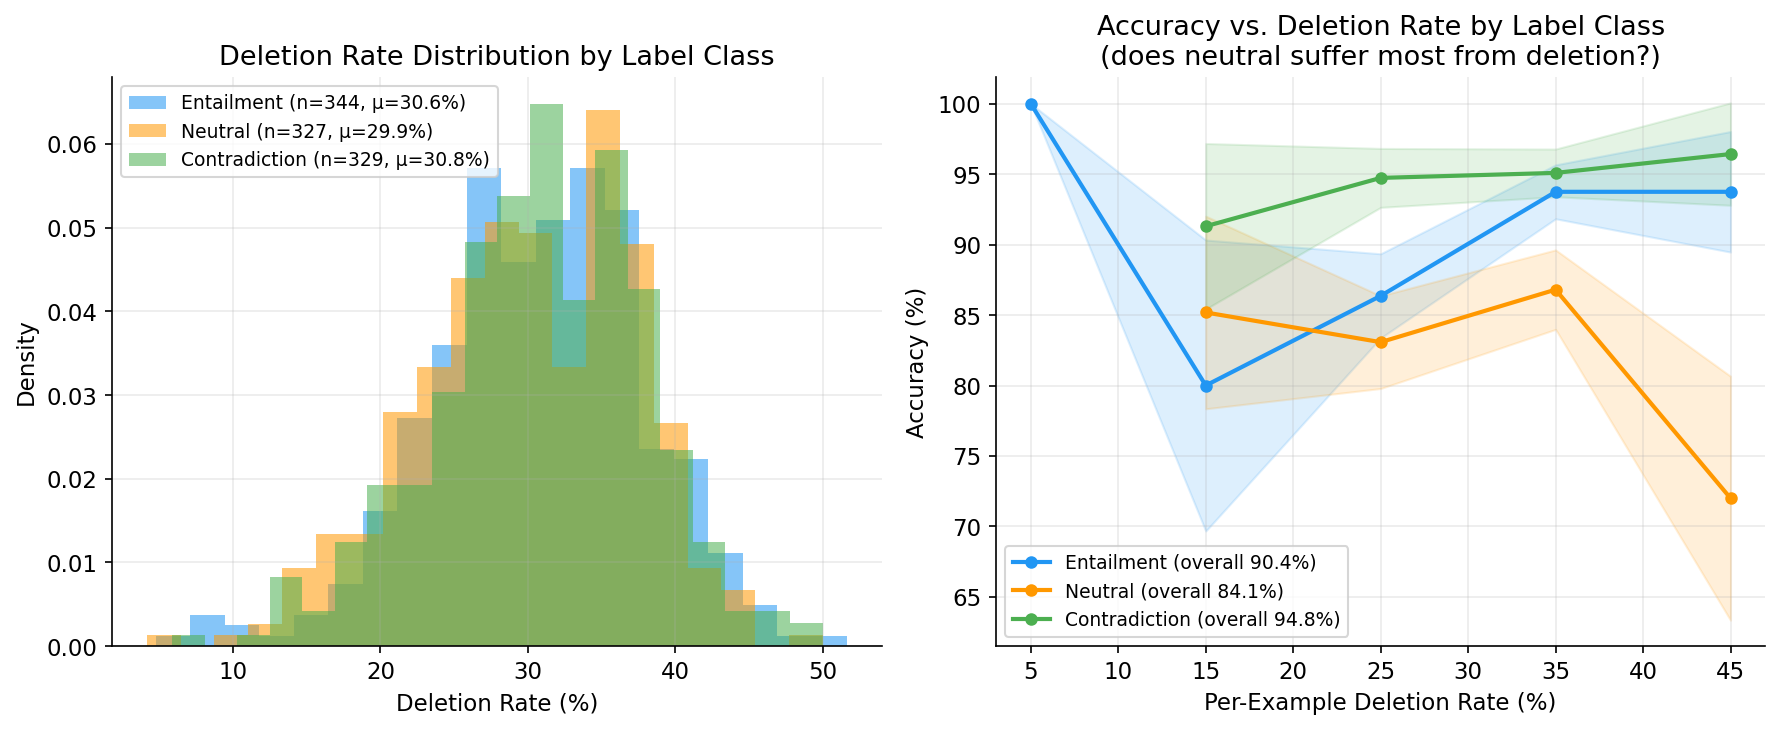
\includegraphics[width=0.55\textwidth]{deletion_by_label.png}
\caption{Gate value distributions and deletion rates broken down by SNLI label. Contradiction examples show the highest accuracy; neutral examples have the lowest, with slightly higher deletion rates.}
\label{fig:deletion-by-label}
\end{figure}


\subsection{Task Sensitivity and Attention Sparsification}
\label{sec:task-sensitivity}

Our empirical observations reveal a clear sensitivity spectrum across tasks:

\begin{itemize}[nosep]
    \item \textbf{High tolerance:} SST-2 ($-$0.62pp at 30\%) and IMDB ($-$0.94pp) --- sentiment depends on a few keywords, making most tokens dispensable.
    \item \textbf{Moderate tolerance:} SNLI ($-$0.27pp at 30\%, $-$2.23pp at 70\%) --- performance degrades linearly with deletion.
    \item \textbf{Low tolerance:} TyDi~QA (EM collapses at 70\% target) and MRPC ($-$17.32pp) --- critical information is distributed across many positions or the training set is too small.
\end{itemize}

From a representation perspective, the gate performs a form of \emph{attention sparsification}: by removing low-signal subwords and reducing cross-token interference, it acts as a dynamic regulariser --- especially when the gold label depends on a small subset of salient tokens. In contrast, when critical information is distributed across many positions (extractive QA, paraphrase detection), this sparsification is harmful: once key spans are pruned, the model cannot re-attend to them in later layers, explaining the catastrophic failure modes on TyDi~QA without blending.



\subsection{PI Controller Dynamics on Long Documents}
\label{sec:imdb-instability}

On long-document tasks such as IMDB (max length 512), we observe notable run-to-run instability in both deletion rates and final accuracy, even with the PI controller active. Per-batch deletion ratios for longer sequences are inherently noisier: a single 512-token example contains far more variance in token importance than a 128-token SNLI pair. The PI controller's smoothing ($\gamma=0.9$) adapts too slowly to these fluctuations, allowing the gate to converge to suboptimal operating points. The actual deletion rate on IMDB (43.7\%) substantially overshoots the 30\% target, unlike SNLI where convergence is tight (30.8\%). This suggests that long-document settings may benefit from more conservative PI parameters --- a lower proportional gain $k_p$ or a longer warmup period --- to match the slower temporal dynamics of gate adaptation on long sequences.


% ══════════════════════════════════════════════════════════
\section{Conclusion}
\label{sec:conclusion}

We have demonstrated that the Dynamic Token Merging delete gate from MrT5 transfers to encoder-only discriminative NLU models. MrBERT learns to selectively delete tokens at controlled rates while preserving task performance. 

\noindent\textbf{Key findings:}

\begin{enumerate}[nosep]
    \item \textbf{Minimal accuracy cost (SNLI)}: MrBERT-30\% retains 90.21\% accuracy --- only 0.27pp below BERT baseline --- at \textbf{1.89$\times$} A100 speedup.
    \item \textbf{Task-dependent robustness}: SST-2 ($-$0.62pp) and IMDB ($-$0.94pp) are highly robust; MRPC ($-$17.32pp) is sensitive, likely due to small dataset size.
    \item \textbf{Learned importance}: gate outperforms random deletion by 2.95pp on SNLI and preferentially deletes function words and premise tokens.
    \item \textbf{PI controller is essential}: without it, the gate runs away to 89\% deletion, dropping accuracy 4.01pp.
    \item \textbf{Pre-deletion blending enables QA}: span EM $0.10\to0.35$ ($3.5\times$); end accuracy matches BERT at layer~9.
    \item \textbf{Soft training $\Rightarrow$ hard inference}: soft--hard gap is only 0.05pp, validating the training design.
    \item \textbf{XLM-R requires tuning}: MrXLMR-0\% itself degrades $-$7.63pp, pointing to training stability issues specific to XLM-R's architecture.
\end{enumerate}

\noindent \textbf{Limitations:}
\begin{itemize}[nosep]
    \item Hard deletion breaks batch uniformity, requiring ragged-tensor handling that complicates deployment.
    \item MRPC's large drop ($-$17.32pp) warrants further investigation --- the small dataset (3.7K examples) may make the joint task + deletion objective difficult to optimise.
    \item MrXLMR exhibits training instability even at 0\% deletion ($-$7.63pp), suggesting XLM-R's SentencePiece tokenisation creates higher information density per token; deleting even one subword can collapse a word's semantics.
    \item SQuAD without pre-deletion blending defaults to 0\% deletion (gate collapse), and QA with blending has only been evaluated on TyDi~QA so far.
    \item Per-example loss--deletion correlations, while informative, are weak; stronger conclusions would require larger evaluation sets and more diverse tasks.
\end{itemize}

\noindent \textbf{Future work:}
\begin{enumerate}[nosep]
    \item \textbf{Fix MrXLMR instability}: longer warmup, frozen backbone, layer-wise lr decay, and careful tuning of the gate learning rate.
    \item \textbf{Apply pre-deletion blending to SQuAD}: extend the mechanism that recovered TyDi~QA performance.
    \item \textbf{Evaluate MRPC with longer training} or a higher regulariser delay to disentangle dataset size effects from deletion sensitivity.
    \item \textbf{XNLI zero-shot cross-lingual evaluation} for MrXLMR to assess whether deletion patterns generalise across languages.
    \item \textbf{Human--rationale alignment}: investigate whether gate-prioritised tokens align with human-annotated rationales (ERASER datasets), assessing interpretability.
    \item \textbf{Advanced control theory}: explore RL-based deletion schedules or learned $\alpha$ trajectories for better stability on long-document tasks like IMDB.
\end{enumerate}


\section*{Team Contributions}

\textbf{Hiva Zaad} (\url{https://github.com/HivaMohammadzadeh1/CS224N-project/}): Implemented MrBERT and MrXLMR architectures, ran SNLI/SST-2/MRPC/IMDB/SQuAD/TyDi~QA experiments on A100, developed pre-deletion blending mechanism, inference runtime benchmarking, per-example deletion analysis, and report writing.

\noindent \textbf{Tianhui (Alina) Huang} (\url{https://github.com/TinaLand/standford_cs224n_project/}): Independent implementation and experiments for MrBERT and MrXLMR, cross-validated results, and report writing.

\noindent \textbf{Aronima Dass} (\url{https://github.com/HivaMohammadzadeh1/CS224N-project/}): Independent implementation and experiments for MrBERT and MrXLMR, cross-validated results, and report writing.


% ══════════════════════════════════════════════════════════
\bibliographystyle{plainnat}
\begin{thebibliography}{99}

\bibitem[Devlin et~al.(2019)]{devlin2019bert}
Jacob Devlin, Ming-Wei Chang, Kenton Lee, and Kristina Toutanova.
{BERT}: Pre-training of deep bidirectional transformers for language understanding.
In \emph{NAACL-HLT}, pages 4171--4186, 2019.

\bibitem[Conneau et~al.(2020)]{conneau2020xlmr}
Alexis Conneau, Kartikay Khandelwal, Naman Goyal, Vishrav Chaudhary, Guillaume Wenzek, Francisco Guzm\'{a}n, Edouard Grave, Myle Ott, Luke Zettlemoyer, and Veselin Stoyanov.
Unsupervised cross-lingual representation learning at scale.
In \emph{Proceedings of the 58th Annual Meeting of the Association for Computational Linguistics (ACL)}, pages 8440--8451, 2020.

\bibitem[Kallini et~al.(2024)]{kallini2024mrt5}
Julie Kallini, Maria Tsimpoukelli, and Phil Blunsom.
{MrT5}: Dynamic token merging for efficient byte-level language models.
\emph{arXiv preprint arXiv:2410.20771}, 2024.

\bibitem[Bowman et~al.(2015)]{bowman2015snli}
Samuel~R. Bowman, Gabor Angeli, Christopher Potts, and Christopher~D. Manning.
A large annotated corpus for learning natural language inference.
In \emph{Proceedings of the 2015 Conference on Empirical Methods in Natural Language Processing (EMNLP)}, pages 632--642, 2015.

\bibitem[Clark et~al.(2019)]{clark2019attention}
Kevin Clark, Urvashi Khandelwal, Omer Levy, and Christopher~D. Manning.
What does {BERT} look at? {A}n analysis of {BERT}'s attention.
In \emph{BlackboxNLP Workshop at ACL}, 2019.

\bibitem[Clark et~al.(2020)]{clark2020tydiqa}
Jonathan~H. Clark, Eunsol Choi, Michael Collins, Dan Garrette, Tom Kwiatkowski, Vitaly Nikolaev, and Jennimaria Palomaki.
{TyDi QA}: A benchmark for information-seeking question answering in typologically diverse languages.
In \emph{Transactions of the Association for Computational Linguistics (TACL)}, 2020.

\bibitem[Conneau et~al.(2018)]{conneau2018xnli}
Alexis Conneau, Ruty Rinott, Guillaume Lample, Adina Williams, Samuel Bowman, Holger Schwenk, and Veselin Stoyanov.
{XNLI}: Evaluating cross-lingual sentence representations.
In \emph{Proceedings of the 2018 Conference on Empirical Methods in Natural Language Processing (EMNLP)}, 2018.

\bibitem[Michel et~al.(2019)]{michel2019heads}
Paul Michel, Omer Levy, and Graham Neubig.
Are sixteen heads really better than one?
In \emph{Advances in Neural Information Processing Systems (NeurIPS)}, 2019.

\bibitem[Voita et~al.(2019)]{voita2019heads}
Elena Voita, David Talbot, Fedor Moiseev, Rico Sennrich, and Ivan Titov.
Analyzing multi-head self-attention: Specialized heads do the heavy lifting, the rest can be pruned.
In \emph{Proceedings of the 57th Annual Meeting of the Association for Computational Linguistics (ACL)}, pages 5797--5808, 2019.

\bibitem[Rajpurkar et~al.(2016)]{rajpurkar2016squad}
Pranav Rajpurkar, Jian Zhang, Konstantin Lopyrev, and Percy Liang.
{SQuAD}: 100,000+ questions for machine comprehension of text.
In \emph{Proceedings of the 2016 Conference on Empirical Methods in Natural Language Processing (EMNLP)}, pages 2383--2392, 2016.

\bibitem[Dolan and Brockett(2005)]{dolan2005mrpc}
Bill Dolan and Chris Brockett.
Automatically constructing a corpus of sentential paraphrases.
In \emph{IWP}, 2005.

\bibitem[Wang et~al.(2019)]{wang2019glue}
Alex Wang, Amanpreet Singh, Julian Michael, Felix Hill, Omer Levy, and Samuel~R. Bowman.
{GLUE}: A multi-task benchmark and analysis platform for natural language understanding.
In \emph{ICLR}, 2019.

\bibitem[Maas et~al.(2011)]{maas2011imdb}
Andrew~L. Maas, Raymond~E. Daly, Peter~T. Pham, Dan Huang, Andrew~Y. Ng, and Christopher Potts.
Learning word vectors for sentiment analysis.
In \emph{Proceedings of the 49th Annual Meeting of the Association for Computational Linguistics (ACL)}, 2011.

\bibitem[Socher et~al.(2013)]{socher2013sst}
Richard Socher, Alex Perelygin, Jean Wu, Jason Chuang, Christopher~D. Manning, Andrew Ng, and Christopher Potts.
Recursive deep models for semantic compositionality over a sentiment treebank.
In \emph{Proceedings of the 2013 Conference on Empirical Methods in Natural Language Processing (EMNLP)}, 2013.

\bibitem[Wolf et~al.(2020)]{wolf2020transformers}
Thomas Wolf, Lysandre Debut, Victor Sanh, Julien Chaumond, Clement Delangue, Anthony Moi, Pierric Cistac, Tim Rault, R\'{e}mi Louf, Morgan Funtowicz, Joe Davison, Sam Shleifer, Patrick von Platen, Clara Ma, Yacine Jernite, Julien Plu, Canwen Xu, Teven Le~Scao, Sylvain Gugger, Mariama Drame, Quentin Lhoest, and Alexander~M. Rush.
Transformers: State-of-the-art natural language processing.
In \emph{EMNLP: System Demonstrations}, 2020.

\bibitem[Lhoest et~al.(2021)]{lhoest2021datasets}
Quentin Lhoest, Cl\'{e}ment Delangue, Patrick von Platen, Thomas Wolf, et~al.
Datasets: A community library for natural language processing.
In \emph{EMNLP: System Demonstrations}, 2021.

\end{thebibliography}



% ══════════════════════════════════════════════════════════
\appendix

\section{Parameter Counts}
\label{app:params}

\begin{table}[h]
\centering
\begin{tabular}{@{}lr@{}}
\toprule
\textbf{Component} & \textbf{Parameters} \\
\midrule
BERT-base / XLM-R-base           & 110M / 277M \\
Gate LayerNorm (weight $+$ bias)  & $2 \times 768 = 1{,}536$ \\
Gate Linear (weights $+$ bias)    & $768 + 1 = 769$ \\
\textbf{Total gate}               & \textbf{2,305} \\
Gate as \% of BERT-base          & 0.0021\% \\
\bottomrule
\end{tabular}
\caption{Gate module parameter counts.}
\label{tab:params}
\end{table}


\section{Compute Budget}
\label{app:compute}

\begin{table}[h]
\centering
\begin{tabular}{@{}lr@{}}
\toprule
\textbf{Experiment group} & \textbf{GPU-hours (A100)} \\
\midrule
SNLI --- 11 runs $\times$ $\sim$2.5h each    & $\sim$27.5h \\
SST-2/MRPC/IMDB --- 6 runs $\times$ $\sim$0.4h & $\sim$2.4h \\
SQuAD --- 2 runs $\times$ $\sim$0.8h          & $\sim$1.6h \\
TyDi~QA --- 11 runs $\times$ $\sim$0.07h      & $\sim$0.8h \\
MrXLMR-SNLI --- 4 runs $\times$ $\sim$2.5h    & $\sim$10h \\
\midrule
\textbf{Total}                                  & $\sim$\textbf{42h} \\
\bottomrule
\end{tabular}
\caption{Estimated compute budget (NVIDIA A100 40GB via Modal).}
\label{tab:compute}
\end{table}


\section{Full MrBERT-SNLI Run Inventory}
\label{app:runs}

\begin{table}[h]
\centering\small
\begin{tabular}{@{}lllcc@{}}
\toprule
\textbf{Run} & \textbf{Name} & \textbf{Purpose} & \textbf{Final Acc.} & \textbf{Del. Rate} \\
\midrule
A & bert-snli-baseline       & BERT baseline              & 90.48\% & 0\% \\
B & mrbert-snli-0pct         & MrBERT 0\% sanity check    & 90.50\% & 0\% \\
C & mrbert-snli-30pct        & Main result, soft training & 90.21\% & 30.8\% \\
D & mrbert-snli-50pct        & Tradeoff curve             & 89.52\% & 52.6\% \\
E & mrbert-snli-70pct        & Tradeoff curve             & 88.25\% & 72.4\% \\
F & mrbert-snli-random30     & Random deletion ablation   & 87.26\% & 49.6\% \\
G & mrbert-snli-nopi         & No PI controller ablation  & 86.47\% & 88.9\% \\
H & mrbert-snli-layer1       & Gate layer ablation        & 90.42\% & 31.0\% \\
I & mrbert-snli-layer6       & Gate layer ablation        & 90.36\% & 33.9\% \\
J & mrbert-snli-layer9       & Gate layer ablation        & 90.22\% & 46.3\% \\
M & mrbert-snli-30pct-hd     & Hard-train ($p=0.5$)       & 90.26\% & 31.1\% \\
\bottomrule
\end{tabular}
\caption{All MrBERT-SNLI runs and their final metrics.}
\label{tab:run-inventory}
\end{table}

\section{Per-Example Deletion Analysis (Combined View)}
\label{app:deletion-analysis}

\begin{figure}[h]
\centering
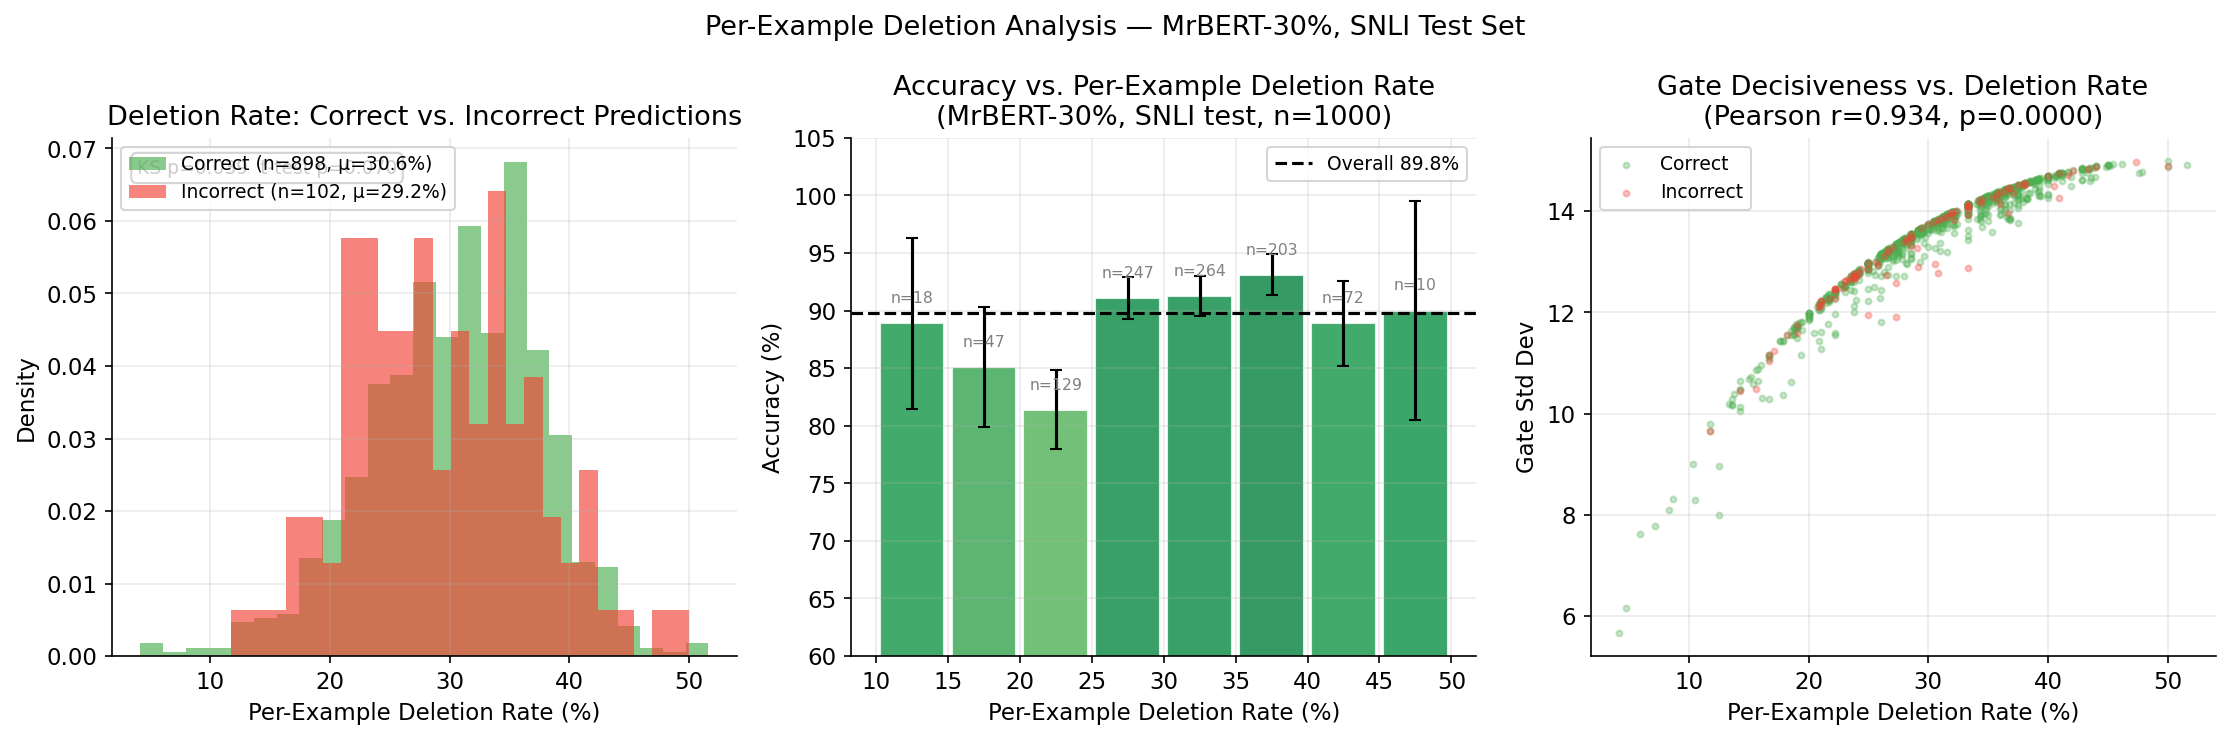
\includegraphics[width=0.85\textwidth]{per_example_deletion_analysis.png}
\caption{Combined per-example deletion analysis on SNLI (MrBERT-30\%, 1,000 examples). The near-flat trend confirms the gate deletes wisely across the full range of deletion rates.}
\label{fig:per-example-combined}
\end{figure}

\end{document}
